\documentclass[a4paper,11pt,oneside,top=3cm,bottom=3cm,left=3.5cm,right=3.5cm,openright,reqno,table]{book}

\linespread{1.5}

\usepackage{listings}
\usepackage{xcolor}

%Permette di usare l'opzione H per forzare una figura in un certo posto
\usepackage{float}

\usepackage{ltablex, ltablex, colortbl}
\keepXColumns
\definecolor{lightgray}{gray}{0.9}


%Multiline comment
\usepackage{verbatim}

\usepackage{svg}

% Carica immagini
\usepackage{graphicx}

\usepackage{url} % Pacchetto per gestire i link

\usepackage{amsmath}
\usepackage{amssymb} % Per utilizzare \mathbb{}
\usepackage[utf8]{inputenc}

% Pacchetti per la formattazione e la lingua
\usepackage[utf8]{inputenc} % Codifica dei caratteri
\usepackage[T1]{fontenc}
\usepackage[italian]{babel}

% Pacchetti per la gestione delle immagini
\usepackage{subcaption}

% Pacchetto per i colori
\usepackage{xcolor}

% Pacchetti per migliorare la lettura e la struttura del documento
\usepackage{microtype}
\usepackage{setspace}
\usepackage{indentfirst}

% Pacchetto per link e riferimenti
\usepackage{hyperref}
\usepackage{bookmark} % Aggiunto pacchetto bookmark

% Pacchetto per la bibliografia
\usepackage{natbib} %Imports biblatex package

% Impostazioni per le dimensioni e i margini della pagina
\usepackage[a4paper, top=2.5cm, bottom=2.5cm, left=3cm, right=2.5cm]{geometry}

% Impostazioni per l'intestazione e il piè di pagina
\usepackage{fancyhdr}
\pagestyle{fancy}
\fancyhf{}
\rhead{\thepage}
\lhead{\nouppercase{\leftmark}}

% Impostazioni per i titoli dei capitoli
\usepackage{titlesec}
\titleformat{\chapter}[display]
{\normalfont\huge\bfseries}{\chaptertitlename\ \thechapter}{20pt}{\Huge}

% Impostazioni per lo stile del codice C
\lstdefinestyle{C}{
  language=C,
  basicstyle=\ttfamily\small,
  numbers=left,
  numberstyle=\tiny,
  numbersep=5pt,
  tabsize=2,
  extendedchars=true,
  breaklines=true,
  keywordstyle=\color{blue},
  stringstyle=\color{red},
  commentstyle=\color{green},
  rulecolor=\color{black},
  xleftmargin=2em,
  xrightmargin=2em,
  aboveskip=1em,
  showstringspaces=false
}

\lstdefinestyle{Go}{
    language=Go,
    basicstyle=\ttfamily,
    keywordstyle=\color{blue},
    commentstyle=\color{green},
    morecomment=[l][\color{magenta}]{\#},
    stringstyle=\color{orange},
    showstringspaces=false,
    numbers=left,
    numberstyle=\tiny,
    numbersep=5pt,
    tabsize=4,
    breaklines=true,
    breakatwhitespace=false,
    morekeywords={struct, json}
}

\lstdefinestyle{bash}{
    language=bash,
    basicstyle=\ttfamily,
    keywordstyle=\color{blue},
    commentstyle=\color{green},
    stringstyle=\color{red},
    showstringspaces=false,
    numbers=left,
    numberstyle=\tiny,
    numbersep=5pt,
    tabsize=4,
    breaklines=true,
    breakatwhitespace=false,
    morekeywords={ls, echo, cd, pwd, exit, if, then, else, fi, for, do, done}
}

\lstdefinestyle{Python}{
  language=Python,
  basicstyle=\ttfamily\small,
  numbers=left,
  numberstyle=\tiny,
  numbersep=5pt,
  tabsize=2,
  extendedchars=true,
  breaklines=true,
  keywordstyle=\color{blue},
  stringstyle=\color{red},
  commentstyle=\color{green},
  rulecolor=\color{black},
  xleftmargin=2em,
  xrightmargin=2em,
  aboveskip=1em,
  showstringspaces=false
}


\begin{document}

% Pagina del titolo
\begin{titlepage}
    \centering
    
\includegraphics[width=0.3\textwidth]{logo_UNISA.png}\par\vspace{1cm}
    {\scshape\LARGE Università degli Studi di Salerno\par}
    \vspace{1cm}
    {\scshape\Large Tesi di Laurea Triennale in Informatica\par}
    \vspace{1.5cm}
    {\huge\bfseries ANALISI E SVILUPPO DI UN MODERNO FILESYSTEM
CRITTOGRAFICO TRASPARENTE PER LINUX: TCFS \par}
    \vspace{2cm}
    {\Large\itshape Carlo Alberto Giordano \\ matr. 0512110442\par}
    \vfill
    Relatore:\par
    Prof.~Giuseppe \textsc{Cattaneo}
    \vfill
    % Data
    {\large 21 Marzo 2024\par}
\end{titlepage}

\pagenumbering{roman}
% Abstract
\chapter*{Abstract}
\addcontentsline{toc}{chapter}{Abstract}

L'obiettivo di questa tesi è analizzare e sviluppare un moderno filesystem crittografico trasparente per il sistema operativo Linux, concentrandosi sul caso di studio di TCFS. Dopo una  valutazione critica degli approcci esistenti, si è proceduto alla progettazione e implementazione di TCFS, integrando l'algoritmo di cifratura AES per garantire la sicurezza dei dati. Questa tesi fornisce una panoramica approfondita dell'analisi e dello sviluppo di TCFS come moderno filesystem crittografico, evidenziando i benefici e le sfide associate alla sua implementazione e offrendo spunti per ulteriori ricerche nel campo della sicurezza informatica e dei sistemi operativi.
% Sommario
\chapter*{Sommario}
\addcontentsline{toc}{chapter}{Sommario}

Il presente lavoro di tesi si propone di analizzare e sviluppare un moderno filesystem crittografico trasparente per il sistema operativo Linux, con particolare attenzione al caso di studio di TCFS. Dopo una breve introduzione al tema e alla motivazione del lavoro, vengono esposti gli obiettivi della ricerca e la metodologia adottata.

Il primo capitolo fornisce alcuni cenni storici su TCFS, esaminando il contesto storico nel quale è nato, la sua prima implementazione e i miglioramenti della nuova versione di TCFS. Si descrive in dettaglio il contesto storico e le motivazioni che hanno portato alla riscrittura totale di TCFS.

Il secondo capitolo fornisce una definizione approfondita di TCFS, esaminandone le caratteristiche principali e il funzionamento. Si descrivono in dettaglio l'architettura del sistema, comprensiva del server REST, del key manager e del client, nonché l'interfaccia con FUSE. Vengono discussi i vantaggi e gli svantaggi di TCFS e le sfide ancora aperte.

Il terzo capitolo approfondisce l'algoritmo di cifratura AES, utilizzato da TCFS per garantire la sicurezza dei dati. Si analizzano le caratteristiche di AES, il processo di cifratura e decifratura dei file, nonché l'integrazione di AES con TCFS, compresa la gestione delle chiavi e la verifica dell'integrità dei file.

Nel quarto capitolo si analizza in dettaglio il processo di lettura e scrittura all'interno di TCFS, si scende in dettaglio e si guarda al codice che gestisce le operazioni di lettura e scrittura, insieme alle operazioni di generazione e gestione delle chiavi.

Nel quinto capitolo, vengono valutate le prestazioni e la sicurezza di TCFS attraverso criteri e metodi di valutazione specifici. Si confronta TCFS con altri filesystem crittografici, si identificano possibili attacchi e si discutono le contromisure adottate. Infine, vengono presentati i risultati dell'analisi e le relative discussioni.

Le conclusioni riassumono i risultati ottenuti, delineando i limiti del lavoro svolto e suggerendo possibili sviluppi futuri. Si offrono anche considerazioni personali e critiche sul processo di ricerca e sviluppo.

Il presente documento si propone quindi di offrire una panoramica completa sull'analisi e lo sviluppo di TCFS come moderno filesystem crittografico trasparente per Linux, con riferimenti agli aspetti di sicurezza, prestazioni e sviluppi futuri.

\pagenumbering{arabic}

% Indici
\tableofcontents
\listoffigures
\listoftables

% Impostazioni per il corpo del testo
\setlength{\parindent}{1.5em}
\onehalfspacing

% Capitoli
\chapter{Cenni storici su TCFS}
Nella sua versione originale TCFS era molto diverso diverso da quello che è oggi, tutte le seguenti considerazioni in questo capitolo sono frutto dell'analisi di un unico documento, una delle ultime tracce rimaste della versione originale di TCFS. Il documento denominato: "The Design and Implementation of a Transparent Cryptographic Filesystem for UNIX" presentato nel 2001 allo USENIX è stato di forte ispirazione per il progetto. Sfortunatamente il codice originale è stato perso, questo ha comportato una ri-scrittura totale del FS.

\section{Il vecchio TCFS: origine e caratteristiche}
TCFS inizia a prendere forma ad UNISA, nel 1995, con lo scopo di rendere sicura la conservazione dei dati su macchine un pò diverse da quelle che abbiamo oggi, si intende dire che i computer erano basati su un’architettura in cui c’era una macchina principale e diversi terminali connessi. Questo era dovuto all’alto costo delle macchine dell’epoca, che rendeva impossibile avere un computer prestante e personale per ogni utente. Ad oggi diamo per scontato che il computer sia personale e che di solito l'utente connesso a una macchina sia singolo. Nella nuova versione di TCFS si sono tenuti in considerazione questi aspetti.

\subsection{Il contesto storico e le motivazioni del progetto}
La protezione dei dati memorizzati sul server era ed è tutt'ora una sfida importante, in quanto il server può essere soggetto a attacchi, guasti, o accessi non autorizzati. Inoltre, la comunicazione tra il client e il server può essere intercettata o alterata da terze parti malintenzionate. Per questi motivi si sentiva la necessità di sviluppare dei filesystem crittografici che potessero garantire la confidenzialità, l’integrità, e l’autenticazione dei dati, sia in transito che in riposo. I filesystem crittografici sono stati oggetto di molte ricerche negli ultimi decenni, a partire dalle prime proposte. Lungo questa linea di ricerca, la trasparenza (il fatto che il filesystem non sia locale dovrebbe essere nascosto alle applicazioni e agli utenti) e la sicurezza sono state le due questioni principali.
Alcuni sistemi, come il Cluster File System di Compaq , garantiscono la trasparenza anche in presenza di guasti, ma assumono che la confidenzialità dei dati e l’autenticazione delle parti coinvolte sia ottenuta attraverso qualche altro sistema.
Il File System di Andrew e CODA invece forniscono dei meccanismi per autenticare i server su linee pubbliche e per assicurare che la comunicazione client-server non possa essere intercettata. Le serie questioni di gestione delle chiavi che sorgono in tali file system sono affrontate dal Self-certifying File System. Facciamo notare che sia AFS che CODA assumono che il server sia affidabile e memorizzano i dati in chiaro sulla macchina server. TCFS invece memorizza i file in forma criptata, negando al server l’accesso ai dati in chiaro.

\subsection{L’architettura e le funzionalità del vecchio TCFS}
Date le tecnologie dell'epoca TCFS era strutturado in maniera completamente diversa rispetto ad oggi. Esso era costituito da un modulo kernel scritto "ad hoc", che si occupava di memorizzare e mantenere in maniera sicura le chiavi degli utenti all'interno del kernel; utilizzava systemcall, anch'esse scritte appositamente per TCFS, per richiedere e salvare le chiavi degli utenti. Inoltre il FS era capace di comunicare solo con NFS, difatti era una versione modificata proprio di NFS.

\subsection{I limiti e le critiche al vecchio TCFS} 
Nonostante TCFS fosse un passo avanti per l'epoca ad oggi appaiono palesi alcune limitazioni date dall'avanzare dei tempi. Con questo si intende che TCFS era limitato alla comunicazione tramite NFS, richiedeva la ri-compilazione del kernel per aggiungere la gestione delle chiavi e richiedeva che le funzioni crittografiche fossero scritte da zero ed internamente al kernel, tutte queste limitazioni sono state superate dalla versione attuale di TCFS. Per quanto riguarda le critiche alla versione originale di TCFS abbiamo che "\textit{TCFS presenta diversi punti deboli che lo rendono meno utile per la distribuzione. In primo luogo, il ricorso alle password di accesso come chiavi utente non è sicuro. Inoltre, la memorizzazione delle chiavi di crittografia su disco in un database di chiavi riduce ulteriormente la sicurezza. Infine, TCFS è disponibile solo su sistemi con kernel Linux 2.2.17 o precedenti, il che ne limita la disponibilità.}"\cite{AnalisiDiDiversiFS}


\section{Il nuovo TCFS: innovazione e sviluppo} 
La nuova versione di TCFS basa la sua implementazione su FUSE, che ha permesso di portare il codice in userspace, utilizzare librerie crittografiche (nel nostro caso fornite da openssl), e di svincolarci da NFS. Di fatti la nuova versione può funzionare insieme a qualsiasi tipo di FS a patto che supporti gli extended attributes. Nella pratica possiamo immaginarlo come un overlay posto al di sopra della cartella sulla quale viene montato TCFS. Lo sviluppo è stato al dir poco travagliato e ha richiesto la costante e continua ricerca delle nuove tecnologie e di come queste potessero essere adattate all'idea proposta. La nuova gestione del keyring di Linux ha permesso di eliminare la necessità di un modulo kernel per la gestione delle chiavi utente, FUSE ha permesso di portare il codice in userspace, MariaDB e GO hanno permesso un implementazzione del threshold sharing semplificata. Il progetto è stato totalmente reinventato.

\subsection{Le ragioni e gli obiettivi della riscrittura del progetto} 
Come specificato precedentemente il codice originale di TCFS è stato perso, per questo motivo si è dovuto riscrivere interamente il FS. Chiaramente dato l'avanzare dei tempi si è ritenuto necessario indagare le nuove tecnologie proposte da quest'epoca, ma si è anche voluto rispettare quanto più possibile il disegno originale, tenendo a mente i seguenti obbiettivi:
\begin{itemize}
    \item \textbf{Portabilità}: Tutte le tecnologie utilizzate da TCFS sono disponibili per OS UNIX-based, cioè Linux, MacOS, NetBSD, OpenBSD, FreeBSD e similari, ma anche per WINDOWS e Solaris, ed è stato scritto in linguaggi portabili, C e GO, rendendo il porting verso nuove architetture plausibile.
    \item \textbf{Semplicità}: TCFS vuole essere semplice nella sua architettura, semplice nel debug e semplice da utilizzare per l'utente.
    \item \textbf{Trasparenza}: La trasparenza in un FS è un concetto fondamentale che richiede una comprensione approfondita. Quando parliamo di trasparenza in un FS, ci riferiamo alla capacità del sistema di nascondere la complessità delle sue operazioni interne all’utente e in questo caso anche al server remoto, rendendo l’interazione con il sistema il più semplice e intuitiva possibile. La creazione di un FS che sia totalmente trasparente all’utente non è un compito semplice per diversi motivi: Le operazioni che un FS esegue in background sono estremamente complesse. Queste includono la gestione dello spazio su disco, l’organizzazione dei file, la gestione dei permessi di accesso, e numerose altre. Nascondere queste operazioni all’utente richiede un design accurato e un’implementazione meticolosa. Quando un FS interagisce con un server remoto, ci sono molte variabili da considerare. Queste includono la latenza della rete, la gestione degli errori di rete, la sincronizzazione dei file tra il client e il server, ecc. Decidere di non applicare modifiche a un server remoto può sembrare una soluzione facile, ma in realtà, raggiungere una trasparenza totale sia verso il server che verso l’utente richiede di tenere conto di queste variabili. Un altro aspetto importante della trasparenza è la gestione degli errori. Un FS deve essere in grado di gestire gli errori in modo tale da minimizzare l’impatto sull’utente. Questo può includere il recupero da errori di sistema, la gestione di errori di rete, la prevenzione della perdita di dati, ecc. Infine, un FS deve essere in grado di fornire un alto livello di performance pur mantenendo la trasparenza. Questo significa che deve essere in grado di gestire grandi quantità di dati, eseguire operazioni in modo efficiente e rispondere rapidamente alle richieste dell’utente. In conclusione, la trasparenza in un FS è un obiettivo difficile da raggiungere a causa della complessità delle operazioni coinvolte e delle sfide associate all’interazione con i server remoti. Tuttavia, con un design accurato e un’implementazione meticolosa, è possibile creare un FS che fornisca un alto livello di trasparenza all’utente.
    \item \textbf{Sostenibilità}: La sostenibilità è un aspetto cruciale nella scrittura di un progetto software. Essa implica la capacità del progetto di resistere nel tempo, adattandosi alle nuove tecnologie e alle esigenze mutevoli degli utenti. La sostenibilità di un progetto software può essere influenzata da vari fattori, tra cui l’uso accurato delle tecnologie disponibili, la manutenibilità del codice e la capacità di adattarsi alle nuove versioni delle dipendenze. Nel caso specifico di TCFS, la versione originale è stata sviluppata come modulo del kernel. Questo significa che ogni volta che viene rilasciata una nuova versione del kernel, è necessario rivedere e potenzialmente aggiornare l’implementazione di TCFS. Questo può rendere la manutenzione del progetto difficile e laboriosa. Tuttavia, la nuova versione di TCFS supera queste limitazioni. Invece di richiedere che il team di TCFS mantenga il modulo del kernel, questa responsabilità viene delegata agli sviluppatori del kernel stesso. Questo significa che, presumibilmente, il modulo del kernel sarà supportato per tutta la sua vita, indipendentemente dalle modifiche al kernel. Questo approccio ha diversi vantaggi. Prima di tutto, riduce il carico di lavoro del team di TCFS, permettendo loro di concentrarsi su altre aree del progetto, non aumentando il carico sugli sviluppatori del kernel. In conclusione, la sostenibilità di un progetto software è un obiettivo importante che può essere raggiunto attraverso un uso accurato delle tecnologie disponibili e un’attenta pianificazione della manutenzione e dell’evoluzione del progetto. Nel caso di TCFS, la delega della manutenzione del modulo del kernel agli sviluppatori del kernel stesso è un esempio di come questo obiettivo possa essere raggiunto a costo zero.
\end{itemize}

\subsection{Le prospettive future del nuovo TCFS}
Al momento di redazione di questa tesi l'implementazione di TCFS risulta incompleta, di fatti non supporta nessun meccanismo di key-recovery e l'implementazione del threshold sharing è parziale, inoltre non è stato svilupparo nessun programma che aiuti l'utente a montare il FS; un altro passo importante è l'utilizzo di funzioni di lettura e scrittura crittografiche che supportino il parallelismo. Ci si prospetta l'implementazione di queste funzionalità nelle versione successive di TCFS. 

\subsection{Il contributo e il valore del nuovo TCFS} 
L’implementazione del nuovo TCFS si colloca in un contesto storico-sociale in cui la salvaguardia dei dati personali è emersa come un problema di rilevanza critica. Questa problematica è particolarmente accentuata nell’attuale era digitale, caratterizzata dalla presenza di conglomerati tecnologici che acquisiscono e analizzano dati personali per scopi di lucro. In questo scenario, la privacy appare come un concetto che rischia di essere trascurato. Come emerge da diverse fonti \cite{4clegal} \cite{altalex1} \cite{altalex2} \cite{cybersecurity360}, le Big Tech sono in grado, attraverso l’utilizzo di strumenti e risorse, capaci di ricavare valore dai dati in loro possesso, di offrire i nostri dati agli advertisers. Tuttavia, questo comporta anche dei rischi e delle sfide, sia per gli utenti che per le autorità, in termini di: diritti e libertà fondamentali della persona; sicurezza e integrità dei dati; concorrenza e mercato; etica e responsabilità.
In questo scenario, il nuovo TCFS offre agli utenti la possibilità di avere il controllo sui propri dati, e di decidere chi e come può accedervi, senza dover rinunciare alla comodità e alla trasparenza di un filesystem tradizionale. In questo modo, il nuovo TCFS contribuisce a rafforzare il principio di protezione delle persone fisiche con riguardo al trattamento dei dati di carattere personale, sancito dal GDPR, e a promuovere una maggiore consapevolezza e gestione dei rischi e della sicurezza legati ai dati.

Uno degli aspetti più importanti e distintivi del nuovo TCFS è la sua capacità di criptare i dati prima di inviarli su un server remoto, tramite protocolli di rete. In questo modo, TCFS garantisce che i dati siano protetti sia in transito che in riposo, cioè sia durante la comunicazione tra il client e il server, sia quando sono memorizzati sul server. Questa funzionalità rende TCFS adatto per l’uso di filesystem di rete, che offrono dei vantaggi, come la condivisione, la scalabilità, e la disponibilità dei dati, ma presentano anche dei rischi, come la perdita, il furto, o la corruzione dei dati, dovuti a possibili attacchi o malfunzionamenti della rete. Con il nuovo TCFS, gli utenti possono usufruire dei servizi offerti dalle grandi aziende tecnologiche, senza dover esporre i propri dati in chiaro, e senza dover affidare la loro confidenzialità a terze parti. In questo modo, il nuovo TCFS tutela la privacy degli utenti, e li rende più indipendenti e sicuri.

\subsection{Le considerazioni personali e le lezioni apprese}
Nell’ambito dell’attuale ecosistema tecnologico, l’insorgere di progetti come TCFS appare non solo appropriato, ma imprescindibile. L’appeal di servizi di hosting gratuiti è indiscutibilmente rilevante, tuttavia, è essenziale riconoscere che in tali contesti, l’utente si trasforma inevitabilmente nel prodotto. È altrettanto rilevante sottolineare che, nonostante l’esistenza di servizi di hosting a pagamento, la riservatezza dei dati non è assicurata in quasi nessuna circostanza. Pertanto, l’integrazione di TCFS in questo scenario si rivela di fondamentale importanza. Grazie alla sua eccezionale facilità d’uso, TCFS può essere adoperato anche da utenti con competenze limitate, offrendo una soluzione semplice ma efficace alle sfide inerenti alla privacy che caratterizzano l’era digitale contemporanea.

L’implementazione di questo progetto, come precedentemente accennato, ha comportato notevoli sfide. Questo è dovuto alla vastità del progetto e alla ricerca delle tecnologie appropriate, che ha richiesto un impegno temporale considerevole. Inoltre, l’implementazione degli algoritmi crittografici di OpenSSL si è rivelata un compito arduo. L’acquisizione della padronanza di tutte le tecnologie coinvolte è stata un’esperienza estremamente arricchente. Concludo questo progetto con una consapevolezza più profonda della complessità di AES, delle sfide relative alla privacy, del kernel Linux e dei linguaggi di programmazione C, Go e SQL.


\chapter{Cos’è TCFS e come funziona} 
TCFS (Transparent cryptografic file system) è un FS crittografico con lo scopo di rendere totalmente trasparente all’utente le operazioni crittografiche sottostanti. Un filesystem crittografico permette all’utente di proteggere i dati rendondoli illegibili ad utenti non autorizzati. Molti FS crittografici richiedono all’utente di eseguire comandi particolari per gestire i file inclusi al loro interno, TCFS evita queste scomodità ed evita di dover ricordare una password per accedere ai contenuti, evitando di compromettere la sicurezza. TCFS sfrutta le funzionalità di FUSE per interporsi nella comunicazione tra userspace e kernel in modo da cifrare e decifrare i contenuti dei file e dei nomi dei file. Questo FS ha lo scopo principale di criptare i dati prima di inviarli su un server remoto, tramite protocolli di rete come NFS o webdav e simili, a patto che supportino gli attributi estesi. In questo modo, TCFS garantisce che i dati siano protetti sia in transito che in riposo, cioè sia durante la comunicazione tra il client e il server, sia quando sono memorizzati sul server. L'architettura di TCFS presuppone che il client sia fidato, ma chiaramente non si fida del server. Un aspetto distintivo, sebbene non primario dell’implementazione di TCFS, basata su FUSE, è la capacità tecnica di cifrare anche file in directory locali. Questo rappresenta un valore aggiunto significativo, poiché estende la protezione dei dati oltre il contesto di rete, garantendo la sicurezza dei dati anche a livello locale. In conclusione, l’approccio adottato da TCFS offre un equilibrio ottimale tra facilità d’uso, versatilità e sicurezza dei dati, rendendolo una soluzione ideale per affrontare le sfide della privacy odierna.

\section{Le differenze tra i filesystem non trasparenti e TCFS}
I filesystem crittografici non trasparenti richiedono che l’utente esegua comandi specifici per gestire i file all’interno del sistema, mentre TCFS (Transparent Cryptographic File System) rende queste operazioni crittografiche completamente trasparenti all’utente. Questa trasparenza offre un equilibrio ottimale tra facilità d’uso, versatilità e sicurezza dei dati.

\subsection{Confronto con CODA}
CODA è un sistema di file distribuito sviluppato presso l’Università di Carnegie Mellon che mira a fornire un sistema di file altamente disponibile e scalabile. A differenza di TCFS, CODA non è progettato specificamente per fornire funzionalità crittografiche, tuttavia, CODA supporta la crittografia per la sicurezza dei dati durante la trasmissione. A differenza di CODA, TCFS assicura che i dati sulla rete e a riposo siano crittografati.
Mentre TCFS si concentra sulla trasparenza delle operazioni crittografiche per l’utente, CODA si concentra sulla fornitura di un sistema di file distribuito robusto e resiliente. CODA utilizza tecniche come la replica dei server e la cache del client per fornire accesso ai file anche quando la rete è instabile o non disponibile.

\subsection{Confronto con AFS}
L’Andrew File System (AFS) è un filesystem distribuito che utilizza un insieme di server fidati per presentare uno spazio dei nomi dei file omogeneo e indipendente dalla posizione a tutte le workstation client. Tuttavia, a differenza di TCFS, AFS non fornisce funzionalità crittografiche trasparenti \cite{AnalisiDiDiversiFS}.

\subsection{Confronto con CFS}
Il Cryptographic File System (CFS) è un altro sistema di file crittografico che fornisce la crittografia a livello di file. A differenza di TCFS, CFS non è progettato per essere completamente trasparente per l’utente. Invece, CFS richiede che l’utente monti esplicitamente il filesystem crittografico e fornisca una chiave di crittografia.
Mentre TCFS si concentra sulla trasparenza delle operazioni crittografiche per l’utente, CFS si concentra sulla sicurezza dei dati. CFS utilizza una chiave di crittografia per crittografare i dati, il che significa che solo gli utenti che conoscono la chiave possono accedere ai dati. In conclusione, sia TCFS che CFS offrono funzionalità uniche e preziose. TCFS si distingue per la sua trasparenza nelle operazioni crittografiche, rendendo facile per gli utenti proteggere i loro dati senza dover gestire direttamente la crittografia. Ambedue offrono un alto livello di sicurezza dei dati, con l’uso di chiavi di crittografia per proteggere l’accesso ai dati, ma TCFS lo fa in maniera trasparente. \cite{AnalisiTCFSeCFS}.

\section{Caratteristiche di TCFS}
TCFS pone come carattiristiche principali:
\begin{itemize}
    \item \textbf{Trasparenza}: TCFS rende la cifratura e la de-cifratura dei file invisibili all’utente, che può usare il filesystem ignaro della complessità sottostante, senza dover inserire password o usare comandi specifici.
    \item \textbf{Sicurezza}: TCFS usa l’algoritmo AES GCM per criptare i file, considerato uno dei più sicuri e diffusi al mondo, usando delle chiavi generate casualmente, in modo da ridurre il rischio di perdita o furto delle chiavi. Inoltre questo algoritmo è spesso utilizzato date le sue ottime performance.
    \item \textbf{Flessibilità}: TCFS si basa su FUSE, una tecnologia che permette di creare e gestire dei filesystem a livello utente, senza dover modificare e ricompilare il kernel del sistema operativo. Questo rende TCFS compatibile con diversi supporti fisici e portabile verso diversi OS Inoltre e permette di personalizzare il filesystem sottostante (riferirsi alla figura \ref{fig:TCFS-flow}) in base alle proprie esigenze. 
\end{itemize}

\section{Funzionamento e architettura di TCFS} 
TCFS è diviso in varie parti, un modulo userspace che si interfaccia con FUSE, un server REST per il threshold sharing e un programma helper che aiuta l'utente ad avviare TCFS. Ogni parte in TCFS è di fatto indipendente dalle altre, di seguito viene illustrata in maggiore dettaglio l'architettura del FS.

\subsection{L'architettura di TCFS e dove si trova nello stack} 
Il modulo TCFS agisce come un intermediario tra l’utente e il modulo kernel di FUSE. Questo posizionamento strategico consente a TCFS di intercettare e gestire le invocazioni dei comandi che operano sui file. Una volta che TCFS ha elaborato le operazioni, le inoltra al kernel, che a sua volta esegue l’operazione corrispondente sul file.

Per illustrare meglio questo processo, consideriamo due esempi comuni: la lettura e la scrittura di un file.
\begin{itemize}
    \item \textbf{Lettura di un file}: Quando un utente tenta di leggere un file, l’invocazione del comando di lettura viene prima intercettata dal modulo kernel  di FUSE (grazie a VFS), che inoltra a TCFS la richiesta di lettura. TCFS quindi decifra il contenuto del file e popola un buffer, preallocato dal modulo kernel, con i dati decifrati. Successivamente vengono restituiti i dati decifrati all’utente.
    \item \textbf{Scrittura di un file}: Analogamente, quando un utente scrive su un file, l’invocazione del comando di scrittura viene intercettata da TCFS, che cifra i dati e inoltra i dati cifrati al modulo kernel di FUSE, che scrive i dati cifrati sul file.
\end{itemize}
In entrambi i casi, TCFS garantisce che i dati siano sempre cifrati quando sono memorizzati sul file, fornendo così una protezione crittografica dei dati. Questo meccanismo di interposizione tra l’utente e il kernel consente a TCFS di fornire un livello aggiuntivo di sicurezza e privacy, proteggendo i dati dell’utente da accessi non autorizzati.
\begin{figure}[H]
    \centering
    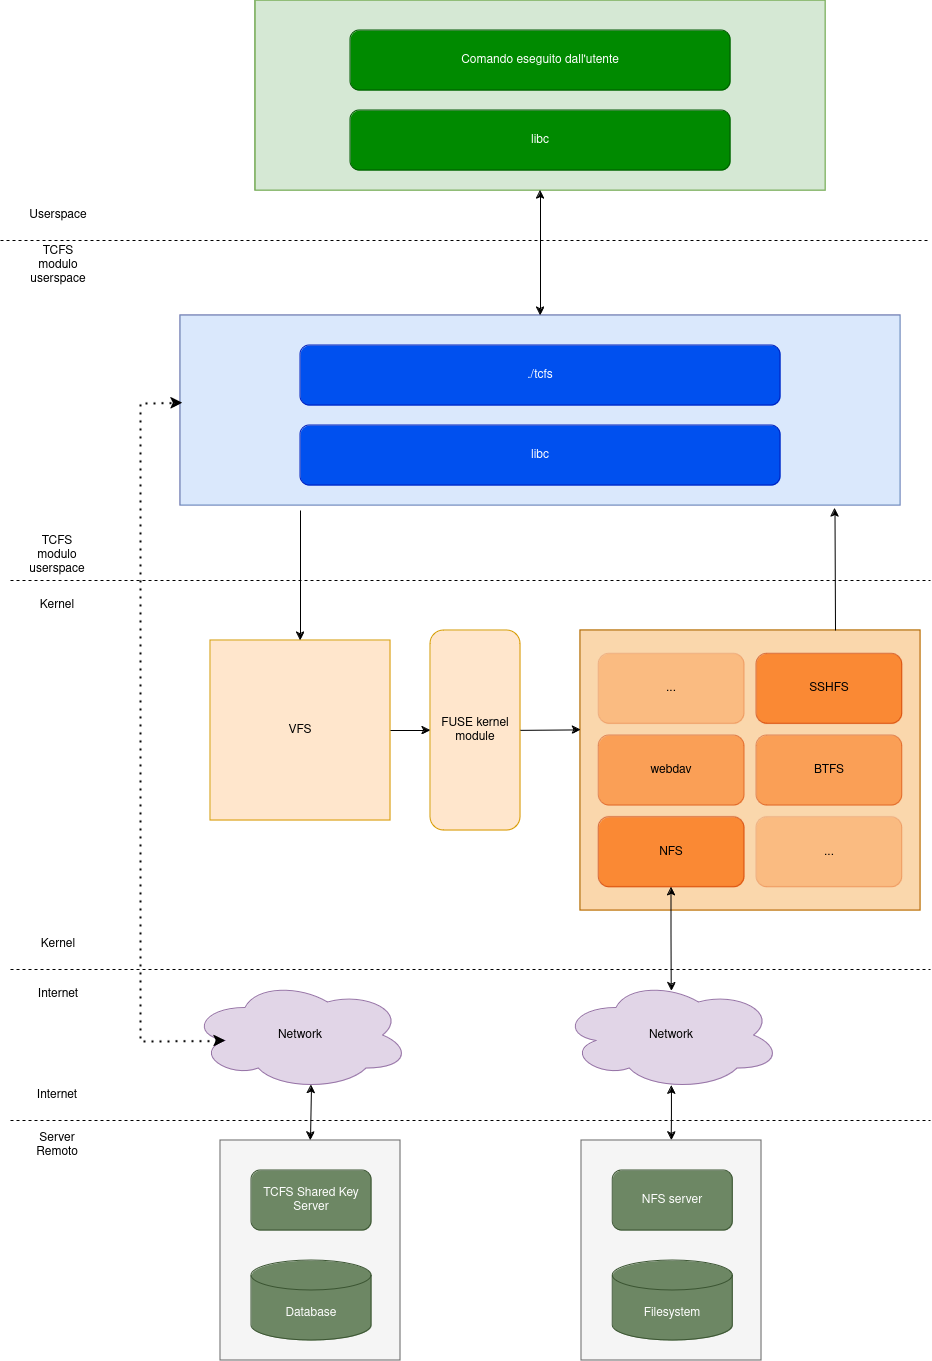
\includegraphics[width=14cm]{capitoli/risorse/TCFSflow.png}
    \caption{Architettura di TCFS}
    \label{fig:TCFS-flow}
\end{figure}

\subsubsection{Chiarimenti su VFS e FUSE}
Il Virtual File System (VFS) è un’interfaccia astratta a livello del kernel del sistema operativo che fornisce un meccanismo per l’interazione uniforme con vari filesystem. Il VFS è responsabile della gestione e coordinamento delle richieste di I/O tra il kernel del sistema operativo e i vari filesystem sottostanti. Esso fornisce un insieme comune di API per le operazioni sui file, indipendentemente dal tipo di filesystem sottostante. Questo livello di astrazione consente al sistema operativo di supportare una vasta gamma di filesystem, come ext4, NTFS, FAT32, ecc., senza dover implementare le specifiche di ciascuno di essi nel kernel.
FUSE (Filesystem in Userspace) è un modulo del kernel che fornisce un’interfaccia per la creazione di filesystem personalizzati in spazio utente. FUSE estende le funzionalità del VFS permettendo agli utenti di implementare un filesystem come un’applicazione a livello di utente, piuttosto che come un modulo del kernel. Questo offre una maggiore flessibilità e sicurezza, poiché gli errori nel codice del filesystem non possono causare crash del sistema.
FUSE si interfaccia con il VFS tramite un’API specifica. Quando un processo effettua una richiesta di I/O su un file o una directory all’interno di un filesystem FUSE, il VFS inoltra la richiesta al modulo FUSE. FUSE a sua volta traduce la richiesta in un formato comprensibile per l’applicazione del filesystem FUSE e la inoltra all’applicazione.
L’applicazione del filesystem FUSE, che è un’applicazione standalone che utilizza la libreria libfuse, implementa la logica specifica del filesystem. Questa applicazione gestisce le richieste provenienti da FUSE, elabora i dati necessari e invia una risposta a FUSE. Ad esempio, se viene richiesta la lettura di un file, l’applicazione del filesystem FUSE leggerà il file dal disco, elaborerà i dati se necessario, e invierà i dati letti a FUSE come risposta.
FUSE quindi restituisce la risposta al VFS, che a sua volta la restituisce al processo che ha effettuato la richiesta originale. In questo modo, FUSE agisce come un ponte tra il VFS a livello di kernel e il filesystem implementato in spazio utente.
In sintesi, il VFS, FUSE e l’applicazione del filesystem FUSE lavorano insieme per fornire un’interfaccia uniforme per la gestione dei filesystem, consentendo al contempo la creazione di filesystem personalizzati in spazio utente. Questo approccio oltre a fornire una grande flessibilità, offre anche un modello di progettazione particolarmente utile, flessibile e semplificato per lo sviluppo di nuovi filesystem, la prototipazione di funzionalità del filesystem e la creazione di filesystem per scopi specifici.

\subsection{Il modulo userspace di TCFS} 
FUSE mette a disposizione una struttura dati che mappa le funzioni specificate da TCFS con le API di FUSE. Nel caso di TCFS le operazioni supportate sono:
\begin{lstlisting}[style=C, caption=Mappa FUSE API alle funzioni di TCFS , label=C-TCFS-FUNCS]
static struct fuse_operations tcfs_oper = {
  .opendir = tcfs_opendir,
  .getattr = tcfs_getattr,
  .access = tcfs_access,
  .readlink = tcfs_readlink,
  .readdir = tcfs_readdir,
  .mknod = tcfs_mknod,
  .mkdir = tcfs_mkdir,
  .symlink = tcfs_symlink,
  .unlink = tcfs_unlink,
  .rmdir = tcfs_rmdir,
  .rename = tcfs_rename,
  .link = tcfs_link,
  .chmod = tcfs_chmod,
  .chown = tcfs_chown,
  .truncate = tcfs_truncate,
  .utimens = tcfs_utimens,
  .open = tcfs_open,
  .read = tcfs_read,
  .write = tcfs_write,
  .statfs = tcfs_statfs,
  .create = tcfs_create,
  .release = tcfs_release,
  .fsync = tcfs_fsync,
  .setxattr = tcfs_setxattr,
  .getxattr = tcfs_getxattr,
  .listxattr = tcfs_listxattr,
  .removexattr = tcfs_removexattr,
};
\end{lstlisting}
Nel contesto di FUSE, quando si parla di funzioni, ci si riferisce alle funzioni di callback che l’utente deve implementare per definire il comportamento del FS. Queste funzioni vengono poi chiamate da FUSE quando si verificano determinate operazioni sul FS, come la lettura di un file o la creazione di una directory.
Ogni funzione di callback ha un insieme specifico di parametri che deve accettare. Questi parametri sono definiti da FUSE e possono includere informazioni come il percorso di un file o la dimensione di un buffer di lettura. Il numero e il tipo di questi parametri sono determinati dalla specifica operazione sul FS che la funzione deve gestire.
Inoltre, FUSE può pre-allocare o pre-riempire alcuni di questi parametri con i dati necessari prima di chiamare la funzione di callback. Ad esempio, se la funzione di callback è responsabile della lettura di un file, FUSE potrebbe pre-allocare un buffer di lettura e passarlo come parametro alla funzione.
In sintesi, FUSE specifica quali parametri una funzione deve accettare e può anche pre-allocare o pre-riempire questi parametri con i dati necessari prima di chiamare la funzione. Questo permette all’utente di concentrarsi sulla logica specifica del FS, senza doversi preoccupare della gestione dei dettagli a basso livello.

\subsection{Il key manager di TCFS} 
TCFS custodisce le chiavi dell'utente all'interno del kernel sfruttando il set di utilities Keyutils, incluso in Linux. Keyutils è un insieme di utility per la gestione e conservazione delle chiavi nel kernel, esso permette di mantenere una chiave all'interno del keyring dell'OS; questa chiave è identificata da in key\_id, che viene specificato nel file di configurazione di TCFS. Il fetch della chiave viene eseguito dall'apposita systemcall keyctl\_read e la chiave viene concessa se e solo se l'ID della chiave è valido e l'utente ha i permessi necessari per richiederla. In generale, l’utente che ha inserito la chiave nel keyring ha i permessi per accedervi, ma può anche concederli o revocarli ad altri utenti, usando il comando keyctl setperm. Chiaramente è necessario ricordare che per definizione dell'architettura di TCFS l'utente è sempre fidato, dunque come abbia ottenuto la chiave non impatta sulla sicurezza del progetto.
Nello specifico è stata sviluppata una libreria denominata key\_utils che espone tre funzioni:
\begin{itemize}
    \item \textbf{char *get\_key ()}:che ottiene la chiave dal kernel e restituisce un buffer contenente la chiave stessa. Il buffer viene allocato dal kernel e condiviso con TCFS.
    \item \textbf{void free\_key (const char *key)}: Che prende in input il puntatore alla chiave, sovrascrive l'area di memoria con "0" e libera lo spazio della chiave.
    \item \textbf{void set\_key\_id(const char *value)}: Che permette di settare l'id della chiave per la sessione attuale di TCFS.
\end{itemize}

\subsection{Il server REST di TCFS} 
Durante il corso del progetto è stato sviluppato un REST in Golang atto a gestire il threshold sharing attraverso l'algoritmo di Shamir. Questo consente di garantire la sicurezza e la riservatezza nell'accesso ai file soggetti al threshold sharing. Si ricorda che questo server non è necessario per il funzionamento di TCFS che ne è di fatti indipendente.
Quando un file viene condiviso utilizzando il threshold sharing la chiave del file viene suddivisa in multiple parti, e ciascuna parte è associata a un share univoco. Il file completo può essere ricostruito solo quando un numero specificato di share viene combinato insieme, rispettando il threshold definito. Non è stato implementato un modo per riottenere la chiave del file.

\subsubsection{Cos'è l'algoritmo di Shamir e come funziona}
Il threshold sharing, ottenuto tramite l'algoritmo di Shamir è un concetto fondamentale nell'ambito della crittografia e della sicurezza informatica. Esso consente di suddividere un segreto in multiple parti, note come "share", in modo che il segreto possa essere ricostruito solo quando un numero minimo di share viene combinato insieme. Questo numero minimo è definito come "threshold". Questa metodologia fornisce un elevato livello di sicurezza, in quanto anche se alcuni share vengono compromessi o ottenuti da parte di terzi non autorizzati, il segreto non può essere ricostruito senza il numero minimo di share richiesto. Pertanto, l'implementazione del threshold sharing tramite l'algoritmo di Shamir nel server REST di TCFS contribuisce in modo significativo alla protezione dei dati e alla sicurezza delle operazioni di accesso ai file.
L'algoritmo di Shamir, fondamentale nell'ambito della crittografia e della sicurezza informatica, si basa sulla matematica dell'interpolazione polinomiale. Per un segreto $S$ l'algoritmo genera un polinomio di grado $(t-1)$, dove $t$ è la soglia. Il termine costante del polinomio è il segreto $S$, mentre gli altri coefficienti del polinomio sono scelti casualmente. Ogni share è quindi un punto $(x, f(x))$ sul polinomio, dove $x$ è un valore unico per ogni share e $f(x)$ è il valore del polinomio calcolato in $x$. Il segreto $S$ può essere ricostruito combinando $t$ share usando l'interpolazione polinomiale di Lagrange.

Più precisamente, l'algoritmo di Shamir procede come segue:

\begin{enumerate}
    \item Scegliamo un numero primo grande $p$ tale che $p > n$ e $p > S$, dove $n$ è il numero totale di share che vogliamo creare.
    \item Creiamo un polinomio di grado $(t-1)$ nel seguente modo:
   \[f(x) = S + a_1x + a_2x^2 + \ldots + a_{t-1}x^{t-1} \mod p\]
   dove $S$ è il termine costante e $a_1, a_2, \ldots, a_{t-1}$ sono coefficienti scelti casualmente.
    \item Ogni share è un punto $(x, f(x))$ sul polinomio, dove $x$ è un valore unico per ogni share e $f(x)$ è il valore del polinomio calcolato in $x$.
    \item Il segreto $S$ può essere ricostruito combinando $t$ share usando l'interpolazione polinomiale di Lagrange. La formula per l'interpolazione di Lagrange è la seguente:
        \[L(x) = \sum_{i=1}^{t} y_i \prod_{1 \leq j \leq t, j \neq i} \frac{x - x_j}{x_i - x_j} \mod p\]
   dove $(x_i, y_i)$ sono le coordinate dei share. Calcolando $L(0)$ otteniamo il segreto $S$.
\end{enumerate}

La sicurezza dell'algoritmo di Shamir si basa sulla difficoltà di risolvere il problema dell'interpolazione polinomiale in presenza di rumore, che è noto come problema di interpolazione di Reed-Solomon. Questo problema è noto per essere NP-hard, il che significa che non esiste un algoritmo efficiente per risolverlo se P $\neq$ NP.

Un problema NP-hard è un problema di decisione per il quale non esiste un algoritmo deterministico che lo risolve in tempo polinomiale. In altre parole, un problema è NP-hard se ogni problema in NP può essere ridotto ad esso in tempo polinomiale. La classe di problemi NP-hard rappresenta quindi i problemi di decisione più difficili in NP. Nonostante la loro difficoltà, i problemi NP-hard sono importanti in quanto forniscono un modo per classificare i problemi computazionali in base alla loro difficoltà intrinseca.


\subsubsection{Registrazione}
Il server si aspetta che ogni utente con il quale si voglia condividere la chiave sia stato registrato. La registrazione avviete tramita una chiamata API a "/register", si specificano il nome utente, la password e la pubkey. Le informazioni vengono deserializzate dal server e salvate nel database, chiaramente non viene salvata la password in chiaro ma un hash della password.

\subsubsection{Login}
Il login all'interno del server è stato implementato ma attualmente non ha nessuna utilità, servirà a riottenere il proprio segreto di Shamir quando sarà terminata l'implementazione del threshold sharing. L'implementazione è molto semplice, l'utente specifica il proprio username e la propria password, quindi il server cerca di eseguire un match con i dati salvati sul database, se questo ha successo allora l'utente viene considerato "loggato" e aggiunto alla tabella corrispondente.

\subsection{Logout}
Il logout avviene in maniera similare al login, viene specificato il nome utente e la password e se sono corretti l'uente viene considerato non più "loggato" e rimosso dalla tabella corrispondente


\subsubsection{Come si condivide un file}
La procedura per richiedere la condivisione di un file si svolge attraverso una chiamata API a “/createSharedFile”. Durante questa chiamata, si specificano due parametri chiave: il numero di share che si desidera generare e il threshold necessario per ricostruire la chiave principale. In risposta a questa richiesta, il server fornisce un ID univoco associato al file, che deve essere conservato all’interno degli attributi estesi del file.
Quando il server riceve questa richiesta, esegue due operazioni fondamentali. Prima di tutto deserializza la richiesta, convertendo i dati in un formato utilizzabile. Successivamente, popola due strutture dati con le informazioni estratte dalla richiesta. Questo processo dettagliato assicura che tutte le informazioni necessarie siano accuratamente raccolte e pronte per l’uso nelle fasi successive del processo di condivisione del file. Segue una breve descrizione del codice:\\ \\

 \begin{lstlisting}[style=Go, caption=Strutture dati ottenute, label=go-structs]
 type User struct {
		Username string `json:"username"`
	}

	type Request struct {
		Users []User `json:"users"`
		K     int    `json:"k"`
	}
\end{lstlisting}
Ottenute queste informazioni si ricostruiscono gli utenti coinvolti nello share grazie al seguente frammento di codice:
 \begin{lstlisting}[style=Go, caption=Ottenimento informazioni utenti, label=go-build-TCFS-USERS]
var users []TCFSTypes.TCFSUser
	for _, user := range req.Users {
		tmpUser := TCFSTypes.TCFSUser{Username: user.Username}
		err := DB.LoadUserInfoByName(&tmpUser)
		if err != nil {
			http.Error(w, err.Error(), http.StatusBadRequest)
			fmt.Printf("Could not load user %v info %v\n", user, err)
			return
		}
		users = append(users, tmpUser)
	}
\end{lstlisting}
Grazie al quale controlliamo se tutti gli utenti che sono coinvolti nello share esistano all'interno del database del server. A questo punto il server procede a generare una chiave chiave, suddividerla tramite Shamir e salvare ogni pezzo della chiave all'interno del suo database, criptandola con la chiave pubblica associata a ogni utente.

\section{Svantaggi e vantaggi di TCFS} %Metti nelle conclusioni vantaggi e svantaggi
Ovviamente TCFS aggiunge un livello di complessità non banale allo share remoto. Gli algoritmi per criptare i file sono molto sicuri, si difendono egragiamente da diversi attacchi, ma questa complessità aggiunge un overhead alla scrittura e lettura dei file, rendendo tutte le operazioni più lente. Questo grande svantaggio viene però compensato dalla sicurezza che tutti i dati presenti sullo share remoto e tutti i dati in transito nella rete siano criptati e indecifrabili per un attaccante.


\section{Sfide e problemi aperti di TCFS} %Conclusioni
Attualmente TCFS non ha grandi problematiche aperte, tuttavia ci sono numerose sfide minori da affrontare. Queste sono:
\begin{itemize}
    \item \textbf{Gestione degli IV}:Attualmente, TCFS non implementa un uso appropriato degli IV nella cifratura dei file. Inoltre, i nomi dei file non utilizzano un IV nel loro processo di cifratura. È importante sottolineare che una corretta gestione degli IV è fondamentale per garantire la sicurezza del sistema. Questo perché l’uso di IV in modo appropriato assicura che la cifratura non sia deterministica, un aspetto cruciale per prevenire attacchi crittanalitici. Pertanto, è essenziale che TCFS rivisiti e migliori la sua gestione degli IV per rafforzare la sicurezza complessiva del sistema.
    \item \textbf{Implementazione del threshold sharing}: Come accennato precedentemente il threshold sharing non è stato implementato completamente. Allo stato attuale non è stata presa nessuna decisione su come ricostruire le chiavi.
    \item \textbf{Parallelismo}: Nessuno degli algoritmi di cifratura di TCFS supporta il parallelismo allo stato attuale del progetto. Una corretta implementazione di questi è di fondamentale importanza per velocizzare le operazioni di IO dal filesystem.
\end{itemize}


\chapter{AES, l’algoritmo di cifratura usato da TCFS}
Nel corso dell'implementazione di TCFS sono stati implementati diversi algoritmi di AES per la cifratura dei file, sono stati valutati CBC, GCM, CTR, e parallelamente, l’AES 256 CBC per la cifratura dei nomi delle cartelle e i nomi dei file. Questo capitolo è dedicato all’analisi delle decisioni progettuali che hanno guidato la selezione di questi algoritmi crittografici e alla discussione dettagliata della loro implementazione all’interno di TCFS. L’obiettivo è di fornire una comprensione approfondita delle motivazioni dietro queste scelte e di come esse contribuiscono a migliorare la sicurezza e l’efficienza del nostro sistema.

\section{Definizione e caratteristiche di AES}
L' \textbf{Advanced Encryption Standard (AES)} è un algoritmo di cifratura a blocchi utilizzato per crittografare dati sensibili. Le sue principali caratteristiche includono:
\begin{itemize}
    \item \textbf{Robustezza}: AES è noto per la sua resistenza agli attacchi crittografici.
    \item \textbf{Efficienza}: L'algoritmo AES è progettato per essere veloce ed efficiente.
    \item \textbf{Flessibilità}: Supporta chiavi di diversi bit (128, 192, 256 bit) offrendo flessibilità nella sicurezza.
    \item \textbf{Standardizzazione}: Essendo uno standard internazionale, AES è ampiamente supportato.
\end{itemize}

\subsection{AES CBC GCM e CTR}
In questa sezione analizzeremo le differenze tra AES CBC, GCM e CTR, i loro vantaggi e svantaggi, e le loro applicazioni per giustificare la scelta implementativa di diffirenziare l'algoritmo di crifratura per i nomi delle cartelle e dei file.

\subsubsection{AES CBC}
AES CBC è un modo di operazione che usa una catena di blocchi per cifrare i dati. Ogni blocco di testo in chiaro viene sottoposto a un’operazione di XOR (OR esclusivo) con il blocco di testo cifrato precedente, o con un vettore di inizializzazione (IV) nel caso del primo blocco, prima di essere cifrato con la chiave AES. Questo modo garantisce che due blocchi uguali di testo in chiaro non producano lo stesso blocco di testo cifrato, aumentando la sicurezza. Tuttavia, AES CBC ha anche alcuni svantaggi:

\begin{itemize} 
\item AES CBC non è parallelizzabile, cioè non è possibile cifrare o decifrare più blocchi contemporaneamente, perché ogni blocco dipende dal precedente. Questo riduce le prestazioni, soprattutto con dati di grandi dimensioni. 
\item AES CBC non fornisce autenticazione, cioè non è possibile verificare se il testo cifrato è stato alterato o manipolato da un attaccante. Si potrebbe usare AES CBC in combinazione con un MAC (Message Authentication Code), che è un codice che garantisce l’integrità dei dati. Questo richiede però una chiave aggiuntiva e un’operazione in più, aumentando la complessità e il costo computazionale. \end{itemize}
AES CBC è adatto per cifrare file locali che non richiedono accesso casuale, cioè che vengono letti o scritti sequenzialmente.

\begin{figure}[h]
    \centering
    \includesvg[width=1\textwidth]{capitoli/risorse/AES_CBC_diagram.svg}
    \caption{Architettura AES CBC}
    \label{fig:AES-CBC-diagramma}
\end{figure}

\subsubsection{AES GCM}
AES GCM è un modo di operazione che usa una modalità contatore per cifrare i dati e una funzione di autenticazione basata sul campo di Galois per garantire l’integrità dei dati. Ogni blocco di testo in chiaro viene sottoposto a un’operazione di XOR con il risultato della cifratura di un contatore, che è un numero che incrementa ad ogni blocco. Il contatore viene inizializzato con un nonce (numero usato una sola volta) e un IV. Il testo cifrato viene poi usato per calcolare un tag di autenticazione, che è un codice che permette di verificare se il testo cifrato è stato alterato o manipolato da un attaccante, il tag in GCM è nella pratica il valore del \textbf{polinomio di Galois}. AES GCM ha diversi vantaggi rispetto a AES CBC:

\begin{itemize} 
\item AES GCM è parallelizzabile, cioè è possibile cifrare o decifrare più blocchi contemporaneamente, perché ogni blocco dipende solo dal contatore. Questo aumenta le prestazioni, soprattutto con dati di grandi dimensioni. 
\item AES GCM fornisce autenticazione, cioè è possibile verificare se il testo cifrato è stato alterato o manipolato da un attaccante. Questo aumenta la sicurezza e la robustezza dell’algoritmo. Inoltre, AES GCM usa la stessa chiave per cifrare e autenticare i dati, riducendo la complessità e il costo computazionale.
\end{itemize}
AES GCM è adatto per cifrare dati che richiedono accesso casuale, cioè che vengono letti o scritti in modo non sequenziale, o che vengono trasmessi su una rete.

\begin{figure}[h]
    \centering
    \includesvg[width=0.7\textwidth]{capitoli/risorse/AES_GCM_diagram.svg}
    \caption{Architettura AES GCM}
    \label{fig:AES-GCM-diagramma}
\end{figure}

\subsubsection{Cos'è il polinomio di Galois}
Il \textbf{polinomio di Galois} è un concetto fondamentale nella teoria dei campi e nell'algebra astratta. Inizialmente introdotto dal matematico Évariste Galois, il polinomio di Galois è associato a ogni estensione di campo finito.
Sia $F$ un campo e $E$ un'estensione di $F$. Se $E$ è un'estensione di Galois, allora il polinomio minimo di un elemento $a \in E$ su $F$ è detto \textbf{polinomio di Galois}.
Ad esempio, consideriamo l'estensione $E = \mathbb{Q}(\sqrt{2})$ su $F = \mathbb{Q}$, dove $\sqrt{2}$ è un numero irrazionale. Il polinomio minimo di $\sqrt{2}$ su $\mathbb{Q}$ è $x^2 - 2$. Questo è anche il polinomio di Galois per l'estensione $E/\mathbb{Q}$.
La teoria dei polinomi di Galois è profonda e ha numerose applicazioni in diverse aree della matematica, come la teoria dei numeri, la crittografia e la teoria dei codici.
Nel nostro caso il polinomio di Galois è utilizzato per generare un'autenticazione di messaggio durante il processo di cifratura e autenticazione dei dati. Questo polinomio è parte integrante dell'algoritmo di autenticazione del messaggio in GCM, che fornisce un modo efficiente per verificare l'integrità dei dati.
Il polinomio di Galois viene utilizzato per moltiplicare i blocchi di dati cifrati con una sequenza di valori di autenticazione derivati da una chiave di autenticazione. Questa operazione produce un'autenticazione dei dati, o MAC, che è inclusa insieme ai dati cifrati per consentire la verifica dell' integrità dei dati.

\subsubsection{AES CTR}
AES CTR (Counter Mode) è un modo di operazione che utilizza un contatore per cifrare i dati. In questo modo, ogni blocco di testo in chiaro viene sottoposto a un’operazione di XOR con il risultato della cifratura di un contatore, che è un numero che incrementa ad ogni blocco. Il contatore viene inizializzato con un nonce (numero usato una sola volta) e un IV. AES CTR incrementa un contatore per ogni blocco successivo cifrato. Ad esempio, se un’applicazione cifra una stringa venti volte di seguito, allora il risultato di ogni iterazione sarà diverso. Questo perché il contatore viene incrementato.

AES CTR ha diversi vantaggi:
\begin{itemize}
    \item \textbf{Parallelismo}: AES CTR è parallelizzabile, cioè è possibile cifrare o decifrare più blocchi contemporaneamente, perché ogni blocco dipende solo dal contatore. Questo aumenta le prestazioni, soprattutto con dati di grandi dimensioni.
    \item \textbf{Padding}: AES CTR non richiede padding. Normalmente, un algoritmo di cifratura a blocchi (AES, Blowfish, DES, RC2, ecc.) emette un output cifrato che è un multiplo della dimensione del blocco (16 byte per AES come esempio). Con la modalità CTR, il numero di byte di output è esattamente uguale al numero di byte di input, quindi non è richiesto alcun padding.
\end{itemize}
Questa modalità ha un grande svantaggio; a differenza di AES GCM, AES CTR non fornisce autenticazione. Questo significa che non è possibile verificare se il testo cifrato è stato alterato o manipolato da un attaccante. Per questa ragione, AES CTR è spesso utilizzato in combinazione con un codice di autenticazione del messaggio, come HMAC, per garantire sia la confidenzialità che l’integrità dei dati, tuttavia in TCFS non è stata implementata questa funzionalità. AES CTR è adatto per cifrare dati che richiedono accesso casuale, cioè che vengono letti o scritti in modo non sequenziale, o che vengono trasmessi su una rete.

\begin{figure}[H]
    \centering
    \includesvg[width=0.7\textwidth]{capitoli/risorse/CTR.svg}
    \caption{Architettura AES CTR}
    \label{fig:AES-CTR-diagramma}
\end{figure}

\subsubsection{Conclusione}
AES CBC, GCM e CTR sono tre modi di operazione di AES che presentano differenze significative in termini di sicurezza, prestazioni e applicazioni. AES GCM è generalmente più sicuro e più veloce di AES CBC, ma richiede una gestione accurata del nonce e dell’IV, che non devono essere riutilizzati per la stessa chiave. AES CBC è più semplice da implementare, ma non è parallelizzabile. AES CTR oltre a essere marginalmente più veloce di GCM offre prestazioni elevate e parallelizzazione, ma richiede una gestione accurata del contatore. Per questi motivi, sia AES GCM che AES CTR sono attualmente disponibili per la cifratura dei file, mentre AES CBC è utilizzato per i nomi delle directory. La scelta tra i tre dipenderà dalle specifiche esigenze dell’utente in termini di sicurezza, prestazioni e gestione delle chiavi.

\subsubsection{Sviluppi futuri e limitazioni attuali}
Attualmente TCFS non savla un IV per la cifratura dei nomi delle directory, questa limitazione è di caratterizzazione temporale, cioè nonostante lo sviluppo del progetto sia durato diversi mesi non si è riusciti a implementare questa funzionalità. Ci si propone quindi di implementarla quanto prima possibile.

\subsubsection{Valutazioni personali}
Attraverso l’analisi della situazione attuale si ricava che i benefici dovuti alla diversificazione degli algoritmi nei precedenti due scenari, si intende la cifratura dei nomi e la cifratura dei file stessi, venga surclassata dalla complessità manutentiva maggiorata.

\chapter{Read e Write in TCFS}
Nel corso di questo capitolo analizzeremmo in dettaglio il funzionamento delle operazioni di scrittura e lettura all'interno del nostro FS; analizzeremo anche la generazione delle chiavi, i design pattern utilizzati e la logica di base, dando un occhiata al codice di TCFS.

\section{Cenni generali sulla lettura e scrittura dei file in TCFS}
Data la quantità di funzioni crittografice e la complessità di alcune di esse, si è scelto di sviluppare una libreria "ad hoc" per semplificare l'utilizzo delle funzioni di cifratura; la libreria denominata crypt-utils funge a questo scopo, essa espone le seguenti funzioni:

\begin{lstlisting}[style=C, caption=Funzioni di crypt-utils, label=C-crypt-utils-functions.h]
#define ENCRYPT true

#define DECRYPT false

#define IV_SIZE 16 //The fixed size of the initialization vector

extern int do_crypt (int mode, FILE *fp, unsigned char **text, int len, unsigned char *key, unsigned char *iv);

void generate_key (unsigned char *destination);

unsigned char *encrypt_string (unsigned char *plaintext, const char *key, int *encrypted_len);

unsigned char *decrypt_string (unsigned char *base64_ciphertext, const char *key);

int is_valid_key (const unsigned char *key);

const char *encrypt_file_name_with_hex (const char *file, const char *key);

const char *decrypt_file_name_with_hex (const char *enc_file, const char *key);

const char *encrypt_path (const char *path, const char *key);

const char *encrypt_path_and_filename (const char *path, const char *key);

const char *decrypt_path (const char *encrypted_path, const char *key);

const char *decrypt_path_and_filename (const char *encrypted_path, const char *key);
extern unsigned char *generate_iv (void);

\end{lstlisting}
Nel corso delle successive sezioni ci concentreremo sul come i file vengono cifrati, dunque ci interesseremo a do\_crypt e generate\_key.

\subsection{La funzione do\_crypt}
Prima di parlare della cifratura e decifratura dei blocchi è necessario specificare che ambedue le operazioni si ottengono tramite l'utilizzo della funzione do\_crypt, che funge da "facade" per le funzioni interne alla libreria:
\begin{itemize}
    \item \textbf{encrypt\_file\_gcm}: Che si occupa di cifrare il testo in chiaro e scriverlo sul file.
    \item \textbf{decrypt\_file\_gcm}: Che legge il file cifrato e restituisce il testo in chiaro.
\end{itemize}
In particolare do\_crypt opera in base allo stato della variabile \textit{mode} che può assumere valore ENCRYPT o DECRYPT. Questo permette di modificare facilmente le funzioni ci cifratura e decifratura su file nascondendo gran parte della complessità che esse comportano.

\subsection{La cifratura dei blocchi}
La funzione interna encrypt\_file\_gcm si occupa della cifratura dei dati e della scrittura di essi su file. La funzione richiede i seguenti parametri:
    \begin{itemize}
        \item \textbf{FILE *fp}: Il puntatore al file sul quale scrivere, da notare che TCFS scrive sempre e solo in "\textit{append}"
        \item \textbf{unsigned char *plaintext}: La stringa contenente il testo da cifrare.
        \item \textbf{unsigned char *plaintext\_len}: La lunghezza del testo.
        \item \textbf{unsigned char *key}: La chiave AES 256 in formato binario.
        \item \textbf{unsigned char *iv}: L'IV del file.
    \end{itemize}
La funzione si occupa di inizzializzare il contesto di libssl e di cifrare la stringa plaintext, ovviamente la stringa viene cifrata mediante la chiave e l'IV. Dunque per ogni blocco la funzione si comprta nel seguente modo: procede a scrivere prima del blocco la dimensione di quest'ultimo, scrive il testo cifrato e infine scrive scrive il TAG di dimensione definita dalla costante TAG\_LEN, che in questa versione è grande esattamente 16 byte. Quest'ultimo ci garantisce l'integrità del blocco scritto poichè al suo interno conserva il valore del polinomio di Galois. Infine ritorna la dimensione del testo cifrato.
Di fatto ogni blocco difrato ha la seguente forma:
\begin{table}[htbp]
        \centering
        \begin{tabular}{|l|l|l|}
            \hline
            Lunghezza del testo cifrato (4 byte) & Testo cifrato & Tag (16 byte)\\
            \hline
        \end{tabular}
        \caption{Descrizione dei blocchi nella WRITE}
    \label{tab:tabella-blocchi-write}
\end{table}

\subsection{La decifratura dei blocchi}
La decifratura viene svolta dalla funzione decrypt\_file\_gcm che si aspetta i seguenti parametri:
 \begin{itemize}
        \item \textbf{FILE *fp}: Il puntatore al file da leggere.
        \item \textbf{unsigned char *key}: La chiave.
        \item \textbf{unsigned char *iv\_len}: L' initialization vector.
        \item \textbf{unsigned char **plaintext}: Un puntatore al buffer che deve contenere il testo una volta decifrato.
    \end{itemize}
La funzione si aspetta questa configurazione dei blocchi all'interno del file:
\begin{table}[htbp]
        \centering
        \begin{tabular}{|l|l|l|}
            \hline
            Lunghezza del testo cifrato (4 byte) & Testo cifrato & Tag (16 byte)\\
            \hline
        \end{tabular}
        \caption{Descrizione dei blocchi nella READ}
    \label{tab:tabella-blocchi-read}
\end{table}

Per decifrare il file la funzione legge la lunghezza del testo cifrato, successivamente legge il testo e il tag e lo decripta tramite la key e l'IV, dunque procede a scrivere il testo in \textit{*plaintext}. La funzione ritorna la lunghezza del testo in chiaro.

\section{L'implementazione della cifratura e della decifratura} 
TCFS Utilizza AES in modalità GCM per cifrare i blocchi dei file. Questo è una combinazione dell'algoritmo di cifratura simmetrica Advanced Encryption Standard (AES) con la modalità di autenticazione Galois/Counter Mode (GCM),  la modalità di funzionamento di questo algoritmo di cifratura è già stato adescritto nel capitolo precedente. Per completezza riportiamo adesso l'implementazione della lettura e della scrittura con AES GCM:
\begin{lstlisting}[style=C, caption=Esempio di decrypt e decrypt con gcm, label=C-gcm-expl]
extern int
decrypt_file_gcm (FILE *fp, unsigned char *key, unsigned char *iv,
                  unsigned char **plaintext, size_t bytes_to_read, off_t offset)
{
  EVP_CIPHER_CTX *ctx = NULL;
  int len;
  volatile int plaintext_len = 0;
  size_t aligned_offset = 0;
  size_t bytes_read = 0L;
  size_t bytes_read_prev = 0L;
  off_t seek_value = 0L;
  unsigned char *ciphertext = NULL;
  unsigned char tag[TAG_LEN];
  *plaintext = NULL;

  if (setjmp (jump_buffer))
    {
      logErr (
          "An error occurred in decrypt_file_gcm! Freeing resources... error");
      if (ctx)
        EVP_CIPHER_CTX_free (ctx);
      if (ciphertext)
        free (ciphertext);
      return false;
    }

  // Get file size
  fseek (fp, 0, SEEK_END);
  long fsize = ftell (fp);
  fseek (fp, 0, SEEK_SET); // same as rewind(f);

  // Align to offset
  if (offset > fsize)
    {
      aligned_offset = offset;
    }
  while (offset > aligned_offset && offset < fsize)
    {
      fread (&seek_value, sizeof (int), 1, fp);
      bytes_read += (unsigned long)sizeof (int);
      fseek (fp, seek_value, SEEK_CUR);
      bytes_read += seek_value;
      fseek (fp, TAG_LEN, SEEK_CUR);
      bytes_read += TAG_LEN;
      aligned_offset += seek_value;
      if (aligned_offset > offset)
        {
          logDebug ("Offset overshoot");
          bytes_read = bytes_read_prev;
          break;
        }
      else if (aligned_offset == offset)
        {
          logDebug ("Offset Found");
          break;
        }
      else
        {
          bytes_read_prev = bytes_read;
        }
    }

  fseek (fp, bytes_read, SEEK_SET);

  while (ftell (fp) < fsize && plaintext_len < bytes_to_read)
    {
      int ciphertext_len;
      fread (&ciphertext_len, sizeof (int), 1, fp);
      if (ciphertext_len < 0){
          handleErrors();
        }

      logDebug ("Allocating ciphertext of size %d", ciphertext_len);
      ciphertext = malloc (ciphertext_len);
      if (!ciphertext)
        {
          handleErrors ();
        }

      fread (ciphertext, sizeof (unsigned char), ciphertext_len, fp);

      fread (tag, sizeof (unsigned char), TAG_LEN,
             fp); // Read the tag from the file

      if (!(ctx = EVP_CIPHER_CTX_new ()))
        {
          handleErrors ();
        }

      if (1 != EVP_DecryptInit_ex (ctx, EVP_aes_256_gcm (), NULL, key, iv))
        {
          handleErrors ();
        }

      if (!EVP_CIPHER_CTX_ctrl (ctx, EVP_CTRL_GCM_SET_TAG, TAG_LEN, tag))
        {
          handleErrors ();
        }

      *plaintext = realloc (*plaintext, plaintext_len + ciphertext_len);
      if (!*plaintext)
        {
          handleErrors ();
        }

      if (1
          != EVP_DecryptUpdate (ctx, *plaintext + plaintext_len, &len,
                                ciphertext, ciphertext_len))
        {
          handleErrors ();
        }
      plaintext_len += len;

      EVP_CIPHER_CTX_free (ctx);

      free (ciphertext);
    }

  return plaintext_len;
}


  extern int
encrypt_file_gcm (FILE *fp, unsigned char *plaintext, size_t plaintext_len,
                  unsigned char *key, unsigned char *iv, off_t offset)
{
  EVP_CIPHER_CTX *ctx = NULL;
  int len;
  int ciphertext_len;
  unsigned char *ciphertext = NULL;
  unsigned char tag[TAG_LEN];

  if (setjmp (jump_buffer))
    {
      logErr (
          "An error occurred in encrypt_file_gcm! Freeing resources... error");
      EVP_CIPHER_CTX_free (ctx);
      if (ciphertext)
        free (ciphertext);
      return false;
    }

  // Align to offset
  off_t aligned_offset = (offset / TAG_LEN) * TAG_LEN;
  fseek (fp, aligned_offset, SEEK_SET);

  if (!(ctx = EVP_CIPHER_CTX_new ()))
    handleErrors ();

  if (1 != EVP_EncryptInit_ex (ctx, EVP_aes_256_gcm (), NULL, key, iv))
    handleErrors ();

  ciphertext = (unsigned char *)malloc (
      plaintext_len + EVP_CIPHER_block_size (EVP_aes_256_gcm ()));
  if (!ciphertext)
    handleErrors ();

  if (1 != EVP_EncryptUpdate (ctx, ciphertext, &len, plaintext, plaintext_len))
    handleErrors ();
  ciphertext_len = len;

  if (1 != EVP_EncryptFinal_ex (ctx, ciphertext + len, &len))
    handleErrors ();
  ciphertext_len += len;

  if (1 != EVP_CIPHER_CTX_ctrl (ctx, EVP_CTRL_GCM_GET_TAG, TAG_LEN, tag))
    handleErrors ();

  fwrite (&ciphertext_len, sizeof (int), 1, fp);

  if (fwrite (ciphertext, sizeof (unsigned char), ciphertext_len, fp)
      != (unsigned long)ciphertext_len)
    {
      handleErrors ();
    }
  if (fwrite (tag, sizeof (unsigned char), TAG_LEN, fp)
      != (unsigned long)TAG_LEN)
    {
      handleErrors ();
    }

  EVP_CIPHER_CTX_free (ctx);
  free (ciphertext);
  return ciphertext_len;
}
\end{lstlisting}
Ora spieghiamo il comportamento delle funzioni:
\subsubsection{decrypt\_file\_gcm}
La funzione decrypt\_file\_gcm è una funzione di decrittografia che utilizza l’algoritmo Galois/Counter Mode (GCM). Questa funzione prende come input un puntatore a un file, una chiave, un vettore di inizializzazione, un puntatore a un puntatore a un array di caratteri, il numero di byte da leggere e un offset. Inizialmente, la funzione inizializza un contesto di cifratura e altre variabili utilizzate per tenere traccia della posizione nel file e della lunghezza del testo in chiaro. Utilizza setjmp per gestire eventuali errori che possono verificarsi durante l’esecuzione della funzione. Se si verifica un errore, la funzione libera le risorse allocate e restituisce 0.
Successivamente, la funzione calcola la dimensione del file e si posiziona all’offset specificato mediante un ciclo. Questo viene fatto per calcolare il punto di salto nel file corrispondente all'offset specificato. Entra in un altro ciclo che continua fino a quando non ha letto tutti i byte richiesti o fino a quando non ha raggiunto la fine del file. In ogni iterazione del ciclo, legge la lunghezza del testo cifrato, il testo cifrato stesso e il TAG di autenticazione dal file.
Dopo aver letto il testo cifrato e il TAG, la funzione inizializza un nuovo contesto di cifratura e imposta la chiave e il vettore di inizializzazione. Imposta anche il TAG di autenticazione utilizzando EVP\_CIPHER\_CTX\_ctrl. Successivamente, decifra il testo cifrato e lo aggiunge al testo in chiaro. Se si verifica un errore durante la decifratura, la funzione gestisce l’errore e libera le risorse allocate.
Infine, alla fine del ciclo, la funzione libera il contesto di cifratura e il testo cifrato e restituisce la lunghezza del testo in chiaro decifrato.
\subsubsection{encrypt\_file\_gcm}
La funzione encrypt\_file\_gcm è utilizzata per crittografare un file utilizzando l’algoritmo di crittografia GCM (Galois/Counter Mode). La funzione inizia inizializzando un contesto di cifratura e alcune variabili. Utilizza setjmp per gestire eventuali errori che possono verificarsi durante l’esecuzione della funzione. Se si verifica un errore, la funzione libera le risorse allocate e restituisce false.
Successivamente, la funzione si posiziona all’offset specificato nel file. Crea un nuovo contesto di cifratura e imposta la chiave e il vettore di inizializzazione. Alloca memoria per il testo cifrato.
La funzione poi crittografa il testo in chiaro e lo aggiunge al testo cifrato. Se si verifica un errore durante la cifratura, la funzione gestisce l’errore e libera le risorse allocate.
Dopo aver cifrato il testo in chiaro, la funzione recupera il tag di autenticazione e scrive la lunghezza del testo cifrato, il testo cifrato e il tag nel file.
Infine, la funzione libera il contesto di cifratura e il testo cifrato e restituisce la lunghezza del testo cifrato. Questa funzione è un esempio di come si può utilizzare l’API OpenSSL per crittografare un file utilizzando l’algoritmo GCM.


\section{Uso di AES CTR per cifrare e decifrare i file}
L'utilizzo di AES CTR è molto simile a GCM con una singola differenza, non viene salvato il TAG dopo il blocco, di fatto i blocchi sul file hanno la seguente forma:\\
\begin{table}[htbp]
        \centering
        \begin{tabular}{|l|l|}
            \hline
            Lunghezza del testo cifrato (4 byte) & Testo cifrato \\
            \hline
        \end{tabular}
        \caption{Descrizione dei blocchi nella READ-WRITE di AES CTR}
    \label{tab:tabella-blocchi-read-write-ctr}
\end{table} \\
Le funzioni di lettura e scrittura sono molto simili alla modalità GCM (a meno del tag) e per questo non vengono riportate.

\subsection{La gerarchia e la generazione delle chiavi in TCFS}
Il FS di TCFS non utilizza la stessa chiave per cifrare ogni file. Quando un nuovo file viene creato e successivamente scritto, TCFS genera una nuova chiave di 32 byte, che viene cifrata tramite la chiave principale di TCFS ed inserita tra gli extended attributes del file. Questa chiave viene creata tramite la funzione generate\_key riportata di sotto:
\begin{lstlisting}[style=C, caption=Esempio di generate\_key, label=C-gen-key-expl]
void generate_key (unsigned char *destination)
{
  for (int i = 0; i < 10; i++)
    {
      int entropy = check_entropy ();
      if (entropy < 128)
        {
          logWarn ("Not enough entropy, creating some...");
          add_entropy ();
        }

      if (RAND_bytes (destination, 32) != true)
        {
          logErr ("Cannot generate key");
          destination = NULL;
        }

      if (strlen ((const char *)destination) == 32)
        break;
    }

  if (!is_valid_key (destination))
    {
      logErr ("ERR: Generated key is invalid\n");
      destination = NULL;
    }
}
\end{lstlisting}
La funzione check\_entropy() si occupa di verificare la presenza di un numero sufficiente di byte in "/dev/urandom" per la creazione della chiave, mentre add\_entropy() affronta un problema più specifico. In particolare, durante la creazione rapida di numerosi file, potrebbe verificarsi una situazione in cui "/dev/urandom" non sia in grado di generare nuovi byte con la stessa velocità. In questo contesto, la funzione add\_entropy() interviene attendendo che il sistema accumuli abbastanza entropia per garantire una generazione adeguata di byte.

\subsubsection{La differenza tra /dev/random e /dev/urandom}
Il dispositivo speciale "/dev/urandom" in ambienti Unix-like fornisce un flusso di dati pseudo-casuali utilizzati per scopi crittografici e di sicurezza.
A differenza di "/dev/random", che potrebbe bloccarsi se non c'è abbastanza entropia disponibile, /"dev/urandom" è progettato per essere un generatore di numeri casuali più rapido e non bloccante, tuttavia nel testing eseguito su TCFS si sono verificate due condizioni che hanno mandato in errore la generazione delle chiavi:
\begin{itemize}
    \item \textbf{La velocità di urandom non era sufficente}: Nonostante sia progettato per essere quanto più veloce possibile è stato notato che si poteva cadere nel caso in cui non erano stati generati abbastanza byte per ottenere una nuova chiave.
    \item \textbf{Non bloccante}: In caso si verifichi la condizione precedente allora il comportamento non bloccante forza urandom a restituire una sequenza più piccola di quella richiesta.
\end{itemize}
Dunque add\_entropy() interviene in situazioni in cui la generazione rapida di file potrebbe esaurire temporaneamente l'entropia disponibile, consentendo al sistema di accumulare entropia sufficiente per garantire una generazione affidabile dei byte necessari. Questo approccio garantisce una gestione efficace dell'entropia durante operazioni ad alta intensità di creazione di file.

\section{Uso di AES CBC per cifrare e decifrare i percorsi}
TCFS utilizza AES CBC per cifrare e decifrare i nomi delle cartelle. Abbiamo già discusso ampliamente di CBC dunque concentriamoci sulle funzioni che lo rendono possibile. Si utilizzano le seguenti funzioni della libreria crypt-utils:    
\begin{lstlisting}[style=C, caption=Funzioni di crypt-utils, label=C-crypt-utils.h]
const char *encrypt_path (const char *path, const char *key);

const char *encrypt_path_and_filename (const char *path, const char *key);

const char *decrypt_path (const char *encrypted_path, const char *key);

const char *decrypt_path_and_filename (const char *encrypted_path,
                                       const char *key);
\end{lstlisting}
chiaramente encrypt\_path e encrypt\_path\_and\_filename funzionano in maniera estamamente similare, la prima cripta il percorso fino alla cartella desiderata e la seconda cripta il percorso fino al file desiderato, lo stesso vale per decrypt\_path e decrypt\_path\_and\_filename.

\subsection{Perchè AES CBC si scontra con la scrittura dei file in FUSE}
Adesso spieghiamo perché si è deciso di non utilizzare CBC per cifrare il contenuto dei file:
AES CBC è un modo di operazione per la crittografia a blocchi che presenta alcune sfide quando viene utilizzato con FUSE. In particolare, il problema principale con l’uso di AES CBC in questo contesto è legato alla natura stessa di CBC. In CBC, ogni blocco di testo in chiaro viene combinato con il blocco di testo cifrato precedente prima di essere cifrato. Questo significa che la cifratura di un blocco dipende da tutti i blocchi precedenti. Pertanto, se si desidera modificare un singolo blocco all’interno di un file, non è possibile semplicemente decifrare e ricifrare quel blocco singolo. Invece, è necessario decifrare e ricifrare tutti i blocchi dal blocco modificato fino alla fine del file. Questo può essere molto inefficiente, soprattutto per file di grandi dimensioni.
Questo problema è particolarmente evidente quando si utilizza FUSE, che consente operazioni di lettura e scrittura a livello di file. Se un’applicazione tenta di scrivere in una posizione arbitraria all’interno di un file, con AES CBC l’intero file deve essere riscritto, il che può comportare un notevole sovraccarico. Inoltre la lettura randomica in AES CBC è semplicemente impossibile se non si decifra l'intero file.
Per questi motivi, AES CBC non è la scelta migliore per la crittografia a livello di directory o filesystem, ed è dunque stato considerato solo per la cifratura dei nomi delle cartelle e dei file.

\subsection{Dettagli implementativi di encrypt\_path\_and\_filename e decrypt\_path\_and\_filename}
Diamo ora un occhiata a encrypt\_path\_and\_filename per capire meglio la sua implementazione:
\begin{lstlisting}[style=C, caption=Funzione encrypt\_path\_and\_filename, label=C-enc-path-filename.h]
const char *encrypt_path_and_filename (const char *path, const char *key)
{
  char *result = NULL;
  char *token, *saveptr;

  // Check if the path is ".", ".."
  if (strcmp (path, ".") == 0 || strcmp (path, "..") == 0)
    {
      // If it is, no encryption is applied
      result = strdup (path);
      if (!result)
        {
          logErr ("Cannot allocate memory");
          exit (EXIT_FAILURE);
        }
      return result;
    }
  // Check if the path is /
  else if (strcmp (path, "/") == 0)
    {
      logDebug ("got root path\n");
      result = malloc (1 * sizeof (char));
      if (result == NULL)
        {
          logErr ("Cannot allocate memory");
          return NULL;
        }
      result[0] = '\0';
    }

  // Copy the original path
  char *path_copy = strdup (path);
  if (!path_copy)
    {
      logErr ("Cannot allocate memory");
      exit (EXIT_FAILURE);
    }

  // Start encryption
  token = strtok_r (path_copy, "/", &saveptr);
  while (token != NULL)
    {
      // Check if the directory is "." or ".."
      if (strcmp (token, ".") == 0 || strcmp (token, "..") == 0)
        {
          // If it is, no encryption is applied
        }
      else
        {
          // Encrypt each part of the path
          const char *encrypted_part = encrypt_file_name_with_hex (token, key);
          logDebug ("\tEncrypted %s --> %s\n", token, encrypted_part);

          // Concatenate to the result string
          if (result == NULL)
            {
              // Check if the first character of encrypted_part is '/'
              if (encrypted_part[0] != '/')
                {
                  result = malloc (strlen (encrypted_part) + 2);
                  if (!result)
                    {
                      logErr ("Cannot allocate memory");
                      exit (EXIT_FAILURE);
                    }
                  strcpy (result, "/");
                  strcat (result, encrypted_part);
                }
              else
                {
                  result = strdup (encrypted_part);
                }
            }
          else
            {
              size_t result_len = strlen (result);
              size_t encrypted_len = strlen (encrypted_part);

              result = realloc (result, result_len + 1 + encrypted_len + 1);
              if (!result)
                {
                  logErr ("Cannot allocate memory");
                  exit (EXIT_FAILURE);
                }

              // Check if the first character of encrypted_part is '/'
              if (encrypted_part[0] != '/')
                {
                  strcat (result, "/");
                }

              strcat (result, encrypted_part);
              logDebug ("Tempresult: %s\n", result);
            }
        }

      // Move to the next part of the path
      token = strtok_r (NULL, "/", &saveptr);
    }

  // Free the memory allocated for the path copy
  free (path_copy);

  return result;
}
\end{lstlisting}

Notiamo innanzitutto che ci sono casi speciali, essa controlla se il percorso del file è uno dei casi speciali “.”, “..” o “/”. In questi casi, non applica nessuna criptazione e restituisce il percorso originale come risultato, dopo averlo copiato con la funzione strdup.
Se il percorso del file non è uno dei casi speciali, la funzione lo copia in una variabile locale 
path\_copy, usando ancora la funzione strdup.
La funzione inizia il processo di criptazione, usando la funzione strtok\_r per dividere il percorso del file in base al carattere “/”. Questo significa che la funzione considera ogni parte del percorso come una directory da criptare separatamente. Per ogni parte del percorso, la funzione controlla se si tratta di una delle directory speciali “.” o “..”. In questo caso, non applica nessuna criptazione e passa alla parte successiva.
Se la parte del percorso non è una directory speciale, la funzione la cripta usando una funzione ausiliaria chiamata encrypt\_file\_name\_with\_hex, che prende in input la parte del percorso e la chiave di criptazione. Questa funzione restituisce una stringa che rappresenta la parte criptata in esadecimale.
La funzione concatena la parte criptata alla stringa result, aggiungendo il carattere “/” se necessario. Se result è ancora NULL, significa che è la prima parte del percorso da criptare, e quindi la funzione la inizializza con la parte criptata. Altrimenti, la funzione usa la funzione realloc per aumentare la dimensione di result e aggiungere la parte criptata alla fine.
La funzione ripete il processo finché non ha esaurito tutte le parti del percorso del file, usando la variabile token per memorizzare la parte corrente e la variabile saveptr per memorizzare il resto del percorso da processare. La funzione libera la memoria allocata per la copia del percorso del file, usando la funzione free e restituisce la stringa result, che contiene il percorso e il nome del file criptati.
La funzione decrypt\_path\_and\_filename funziona esattamente allo stesso modo ma invece di invocare la funzione ausiliaria encrypt\_file\_name\_with\_hex viene invocata la decrypt\_file\_name\_with\_hex.

\subsection{Le funzioni ausiliarie encrypt\_file\_name\_with\_hex e decrypt\_file\_name\_with\_hex}
Queste due funzioni fungono da facade per le funzioni encrypt\_string e decrypt\_string. analizziamole semparatamente.

\subsubsection{La funzione encrypt\_string}
Questa funzione ha lo scopo di inizializzare il contesto di AES CBC, criptare una stringa di lunghezza arbitraria e restituisce la stringa criptata in esadecimale. Diamo anche qui un occhiata alla sua implementazione:
\begin{lstlisting}[style=C, caption=Funzione encrypt\_string, label=C-key-utils.h]
unsigned char *encrypt_string (unsigned char *plaintext, const char *key,
                int *encrypted_key_len)
{
  EVP_CIPHER_CTX *ctx;
  const EVP_CIPHER *cipher = EVP_aes_256_cbc ();
  unsigned char iv[AES_BLOCK_SIZE];
  memset (iv, 0, AES_BLOCK_SIZE);

  ctx = EVP_CIPHER_CTX_new ();
  if (!ctx)
    {
      return NULL;
    }

  EVP_EncryptInit_ex (ctx, cipher, NULL, (const unsigned char *)key, iv);

  size_t plaintext_len = strlen ((const char *)plaintext);
  unsigned char ciphertext[plaintext_len + AES_BLOCK_SIZE];
  memset (ciphertext, 0, sizeof (ciphertext));

  int len, total_len = 0;
  EVP_EncryptUpdate (ctx, ciphertext, &len, plaintext, (int)plaintext_len);
  total_len += len;
  EVP_EncryptFinal_ex (ctx, ciphertext + total_len, &len);
  total_len += len;
  EVP_CIPHER_CTX_free (ctx);

  unsigned char *encoded_string = malloc (total_len * 2 + 1);
  if (!encoded_string)
    {
      logErr ("Cannot allocate memory for encrypt_string encoded_string");
      return NULL;
    }

  for (int i = 0; i < total_len; i++)
    {
      sprintf ((char *)&encoded_string[i * 2], "%02x", ciphertext[i]);
    }
  encoded_string[total_len * 2] = '\0';

  *encrypted_key_len = total_len * 2;
  return encoded_string;
}
\end{lstlisting}
Per iniziare, la funzione crea una struttura che contiene le informazioni necessarie per la criptazione, come il tipo di metodo AES, la parola chiave e il valore casuale. Questa struttura si chiama contesto di criptazione e viene inizializzata con le funzioni apposite. Successivamente la funzione calcola la lunghezza della frase da criptare e crea un vettore di byte che ha abbastanza spazio per contenere il codice segreto. Dopo, la funzione inizia a criptare la frase e a scrivere il codice segreto nel vettore di byte, usando le funzioni di criptazione. Queste funzioni prendono il contesto di criptazione, la frase e il vettore di byte e restituiscono il numero di byte scritti. La funzione tiene conto di questo numero per sapere quanto è lungo il codice segreto.
Infine, la funzione libera la memoria occupata dal contesto di criptazione e converte il codice segreto in una stringa di caratteri esadecimali. Questo significa che ogni byte viene rappresentato da due cifre da 0 a 9 e da A a F. La funzione restituisce questa stringa, che è il risultato della criptazione.

\subsubsection{La funzione decrypt\_string}

\begin{lstlisting}[style=C, caption=Funzione decrypt\_string, label=C-dec-string.h]
unsigned char *
decrypt_string (unsigned char *ciphertext, const char *key)
{
  EVP_CIPHER_CTX *ctx;
  const EVP_CIPHER *cipher = EVP_aes_256_cbc ();
  unsigned char iv[AES_BLOCK_SIZE];
  memset (iv, 0, AES_BLOCK_SIZE);

  ctx = EVP_CIPHER_CTX_new ();
  EVP_DecryptInit_ex (ctx, cipher, NULL, (const unsigned char *)key, iv);

  size_t ciphertext_len = strlen ((const char *)ciphertext) / 2;
  unsigned char *decoded_ciphertext = malloc (ciphertext_len);

  if (!decoded_ciphertext)
    {
      logErr ("Cannot allocate memory for decrypt_string decoded_ciphertext");
      return NULL;
    }

  for (size_t i = 0; i < ciphertext_len; i++)
    {
      char hex[3]
          = { (char)ciphertext[i * 2], (char)ciphertext[i * 2 + 1], '\0' };
      char *endptr;
      unsigned long byte = strtoul (hex, &endptr, 16);

      if (*endptr != '\0' || byte > UCHAR_MAX)
        {
          logErr ("decrypt string error");
          free ((void *)decoded_ciphertext);
          return NULL;
        }
      decoded_ciphertext[i] = byte;
    }

  unsigned char plaintext[ciphertext_len + AES_BLOCK_SIZE + 1];
  memset (plaintext, 0, sizeof (plaintext));

  int len;
  EVP_DecryptUpdate (ctx, plaintext, &len, decoded_ciphertext,
                     (int)ciphertext_len);
  int padding_len;
  EVP_DecryptFinal_ex (ctx, plaintext + len, &padding_len);
  EVP_CIPHER_CTX_free (ctx);

  unsigned char *decrypted_string
      = (unsigned char *)malloc (len + padding_len + 1);

  if (!decrypted_string)
    {
      logErr ("Cannot allocate memory for decrypt_string decrypted_string");
      return NULL;
    }

  memcpy (decrypted_string, plaintext, len + padding_len);
  decrypted_string[len + padding_len] = '\0';

  free (decoded_ciphertext);

  return decrypted_string;
}
\end{lstlisting}
Per decriptare il codice segreto, la funzione deve prima convertirlo in un vettore di byte, cioè una sequenza di byte che può essere manipolata da libssl. Per fare questo, la funzione usa un ciclo for che scorre la stringa esadecimale e prende ogni coppia di caratteri. Poi, usa la funzione strtoul per convertire la coppia di caratteri in un valore numerico, interpretando la stringa come un numero esadecimale. Se la conversione ha successo, la funzione assegna il valore numerico al byte corrispondente nel vettore di byte. Se la conversione fallisce o il valore numerico è troppo grande per essere contenuto in un byte, la funzione restituisce un errore e termina.
Dopo aver convertito il codice segreto in un vettore di byte, la funzione deve creare una struttura che contiene le informazioni necessarie per la decrittazione, come il tipo di metodo AES, la parola chiave e il valore casuale. Questa struttura si chiama contesto di decrittazione e viene usata dalle funzioni di decrittazione per eseguire le operazioni inverse di quelle fatte dalla criptazione. Il tipo di metodo AES è una costante che indica il tipo di cifrario AES da usare (in questo caso AES-256-CBC, che significa che usa una chiave di 256 bit e una modalità di operazione a blocchi concatenati). La parola chiave è una stringa che rappresenta la chiave segreta di decrittazione, che deve essere la stessa usata per la criptazione. Il valore casuale è un vettore di byte che rappresenta il vettore di inizializzazione, che è un valore usato per rendere più sicura la decrittazione. In questo caso, il vettore di inizializzazione è inizializzato con tutti zeri, usando la funzione memset.
Per inizializzare il contesto di decrittazione, la funzione usa due funzioni apposite: EVP\_CIPHER\_CTX\_new e EVP\_DecryptInit\_ex. La prima funzione crea un nuovo contesto di decrittazione e restituisce un puntatore alla struttura. La seconda funzione inizializza il contesto di decrittazione con il tipo di metodo AES, la parola chiave e il vettore di inizializzazione.
Dopo aver inizializzato il contesto di decrittazione, la funzione deve creare un vettore di byte che ha abbastanza spazio per contenere la frase decrittata. Il vettore di byte ha una dimensione pari alla lunghezza del codice segreto diviso due (perché ogni byte corrisponde a due caratteri esadecimali) più la dimensione di un blocco AES (16 byte), per garantire che ci sia abbastanza spazio per contenere la frase decrittata. Il vettore di byte viene riempito con dei valori nulli, usando la funzione memset, per evitare che ci siano dei dati inutili.
Poi, la funzione inizia a decrittare il codice segreto e a scrivere la frase nel vettore di byte, usando le funzioni di decrittazione. Queste funzioni sono EVP\_DecryptUpdate e EVP\_DecryptFinal\_ex. La prima funzione decritta una parte del codice segreto e la scrive nel vettore di byte, restituendo il numero di byte scritti. La seconda funzione decritta la parte finale del codice segreto e la scrive nel vettore di byte, restituendo il numero di byte scritti. La funzione tiene conto di questi numeri per sapere quanto è lunga la frase decrittata.
Infine, la funzione libera la memoria occupata dal contesto di decrittazione, usando la funzione EVP\_CIPHER\_CTX\_free, e copia la frase dal vettore di byte in una stringa di caratteri, usando la funzione malloc per allocare la memoria e la funzione memcpy per copiare i dati. Questa stringa viene terminata con il carattere '\textbackslash 0', che indica la fine della frase. La funzione restituisce questa stringa, che è il risultato della decrittazione.

\chapter{Analisi delle prestazioni} 
In questo capitolo andiamo ad analizzare le prestazioni di TCFS, comparandola con altri FS.

\section{Il Server per il Testing} Come precedentemente menzionato, TCFS è progettato principalmente per essere utilizzato in combinazione con un filesystem di rete. Per tutti i test, utilizzeremo NFS, che interagirà con BTFS, il filesystem utilizzato dal server remoto. Ecco come NFS interagisce con BTFS:
\begin{itemize}
    \item \textbf{Montaggio del Filesystem}: Un client NFS, per accedere ai file su un server NFS, deve prima “montare” il filesystem remoto. Questo processo associa un punto di montaggio locale (una directory o cartella) al filesystem remoto.
    \item \textbf{Richiesta di File}: Quando un’applicazione sul client NFS richiede un file che risiede sul filesystem NFS montato, il client NFS invia una richiesta al server NFS. Questa richiesta include il percorso del file come appare nel punto di montaggio locale.
    \item \textbf{Interazione con il Filesystem Sottostante}: Il server NFS riceve la richiesta e la traduce in un’operazione sul suo filesystem locale. Ad esempio, se la richiesta era di leggere un file, il server NFS apre il file sul suo filesystem locale e legge i dati richiesti.
    \item \textbf{Risposta al Client}: Il server NFS invia una risposta al client NFS con i dati richiesti (se la richiesta era di leggere un file) o con una conferma dell’operazione (se la richiesta era di scrivere su un file o di modificare i metadati di un file).
    \item \textbf{Visualizzazione dei Dati}: Il client NFS riceve la risposta e la presenta all’applicazione che ha fatto la richiesta come se i dati fossero stati letti da un file locale.
    \end{itemize}
Per quanto riguarda le specifiche del server, abbiamo utilizzato una macchina remota equipaggiata con 12 dischi Seagate BarraCuda da 1 TB (ST1000DM010) ciascuno, da 6 GBit/s, 3,5", 7.200 RPM, con 64 MB di cache, configurati in RAID 10 (Mirror + Stripe) che ci garantisce una velocità di 12x in lettura e 6x in scrittura, fornendo così circa 6 TB di spazio. La macchina dispone di 10 core a 4.6 GHz, 64 GB di RAM (in quad channel) e una connessione Gigabit.

\section{La macchina client}
Tutti questi test verranno eseguiti su una macchina client Huawei D15 2020, con un processore Ryzen 5 3500U, con 4 core, 8 thread, un Max. Boost Clock fino a 3.7GHz, un TDP di 15 Watt e con 8GB di RAM. Tutti i test verranno svolti su OS Fedora 39, utilizzando la versione del kernel Linux 6.7.4-200.fc39.x86\_64. Tutte le operazioni di lettura e scrittura verranno eseguite sul server tramite NFS con una velocità di connessione di 500 Mb/s.

\section{Criteri e metodi di valutazione} 
Per il benchmarking della velocità del filesystem, si prevede di testare sia la lettura che la scrittura sequneziale e randomica. Verranno valutati i Mb/s, il carico sulla CPU complessivo e il throughput.

\subsection{Lettura e Scrittura}
Le operazioni di lettura e scrittura saranno sottoposte a un’analisi dettagliata, utilizzando file e blocchi di dimensioni variabili. Prevediamo di testare file che variano da 1MB a 100MB e blocchi che vanno da 1KB a 16MB. Queste dimensioni non sono state scelte a caso, ma sono state selezionate “\textit{cum grano salis}”. Questo perché le dimensioni dei blocchi possono avere un impatto significativo sulle prestazioni del filesystem: blocchi più piccoli possono portare a un utilizzo più efficiente dello spazio su disco, ma possono anche causare un overhead maggiore a causa del numero maggiore di operazioni di I/O necessarie. D’altra parte, blocchi più grandi possono migliorare le prestazioni di lettura e scrittura sequenziali, ma possono portare a uno spreco di spazio su disco se i file sono significativamente più piccoli della dimensione del blocco.

Per ogni file, testeremo le operazioni con almeno tre dimensioni diverse per i blocchi. Le operazioni di lettura e scrittura verranno eseguite sia in sequenza che in modo casuale, registrando le metriche di ciascuna operazione. Questo processo sarà ripetuto più volte per ottenere una media affidabile. In questo modo, saremo in grado di comprendere meglio come le dimensioni dei blocchi influenzano le prestazioni del filesystem in vari scenari di utilizzo.

\subsection{Il programma di testing}
Si è deciso di sviluppare un tool di benchmarking personalizzato, specificamente progettato per il testing dei filesystem. Questo strumento è stato implementato in Python, un linguaggio noto per la sua leggibilità e flessibilità. La scelta di Python non è casuale: la sua sintassi intuitiva e la sua struttura semplificata rendono il codice facilmente accessibile, quasi come se fosse stato progettato con l’utente meno brillante in mente. Il codice del tool, che verrà presentato di seguito, è commentato. Questo approccio, che evita di sovraccaricare il lettore con dettagli tecnici superflui, facilita la comprensione del suo funzionamento. Il tool di benchmarking è in grado di raccogliere una vasta gamma di metriche. Tuttavia, per lo scopo di questo studio, abbiamo scelto di concentrarci solo su un sottoinsieme di queste metriche, ritenute più rilevanti per la nostra analisi. Questa scelta riflette una filosofia ben nota nel mondo Python: “There should be one-- and preferably only one --obvious way to do it”. Tuttavia, è interessante notare come questa filosofia, pur essendo un pilastro della comunità Python, non sempre trovi una perfetta corrispondenza nella realtà. Infatti, chiunque abbia avuto a che fare con Python sa che, nonostante la sua apparente semplicità, il linguaggio può riservare sorprese. Questo non è un giudizio sul linguaggio in sé, ma piuttosto un invito a considerare che ogni strumento ha i suoi punti di forza e le sue sfide. E Python, nonostante tutte le sue virtù, non fa eccezione. In effetti, potrebbe quasi sembrare che Python, con la sua promessa di un solo modo ovvio per fare le cose, stia in qualche modo giocando un brutto scherzo ai suoi utenti. Ma, come si suol dire, “ogni rosa ha le sue spine”.
% String Formatting: ci sono diverse maniere per formattare le stringhe. Il %, .format(), le f-stringhe. PYTHON MA DI CHE PARLI
% Creazione di Liste: Ci sono diversi modi per creare una lista in Python, ad esempio usando un ciclo for, una list comprehension, o  list()
% Esistenza di un Elemento in un Dizionario: usando l’operatore in, il metodo .get(), o il metodo .has_key().
% Se leggi questo sai perchè lo disprezzo
\begin{lstlisting}[style=Python, caption=Script Python per il benchmarking, label=python-benchmark.py]
import os
import time
import random
import threading
import ctypes
import psutil

# Define constants for posix_fadvise
POSIX_FADV_NORMAL = 0
POSIX_FADV_RANDOM = 1
POSIX_FADV_SEQUENTIAL = 2
POSIX_FADV_WILLNEED = 3
POSIX_FADV_DONTNEED = 4
POSIX_FADV_NOREUSE = 5

# Fetch a reference to posix_fadvise
libc = ctypes.CDLL('libc.so.6')
posix_fadvise = libc.posix_fadvise
posix_fadvise.argtypes = [ctypes.c_int, ctypes.c_int64, ctypes.c_int64, ctypes.c_int]
posix_fadvise.restype = ctypes.c_int

# Function to dump the system cache for a specific file
def drop_cache(file_name):
    fd = os.open(file_name, os.O_RDONLY)
    try:
        res = posix_fadvise(fd, 0, 0, POSIX_FADV_DONTNEED)
        if res != 0:
            raise OSError(res, os.strerror(res))
    finally:
        os.close(fd)

# Function to convert size from string to bytes
def convert_size(size):
    if size.endswith('K'):
        return int(size[:-1]) * 1024
    elif size.endswith('M'):
        return int(size[:-1]) * 1024 * 1024
    elif size.endswith('G'):
        return int(size[:-1]) * 1024 * 1024 * 1024
    else:
        return int(size)

# File size
file_size = convert_size('100M')
# Block size
block_size = convert_size('16M')
# Shared variables
blocks_processed = 0
total_blocks = file_size // block_size
# Generate a block of random data once
random_data = bytearray(os.urandom(block_size))
stop_thread = False

def change_random_data():
    global random_data, stop_thread
    while not stop_thread:
        # Read a random byte from /dev/urandom
        try:
            with open('/dev/urandom', 'rb') as f:
                while True:
                    random_byte = f.read(block_size)
                    if len(random_byte) != block_size:
                        # If no data is read, wait and try again
                        time.sleep(0.5)
                        continue
                    else:
                        # Change a random byte in the block
                        index = random.randint(0, block_size - 1)
                        random_data[index] = random_byte[0]
                        break
        except IOError:
            print("Could not read from /dev/urandom.")

# Start the thread that changes random_data
change_thread = threading.Thread(target=change_random_data)
change_thread.start()

def write_sequential(file_name):
    global blocks_processed
    start_time = time.time()
    with open(file_name, 'wb') as f:
        for _ in range(total_blocks):
            f.write(random_data)  # Use the pre-generated random data
            blocks_processed += 1
    end_time = time.time()
    elapsed_time = end_time - start_time
    speed = file_size / elapsed_time / (1024 * 1024)  # Convert to MB/s
    return elapsed_time, speed

def read_sequential(file_name):
    global blocks_processed
    start_time = time.time()
    with open(file_name, 'rb') as f:
        while f.read(block_size):
            blocks_processed += 1
    end_time = time.time()
    elapsed_time = end_time - start_time
    speed = file_size / elapsed_time / (1024 * 1024)  # Convert to MB/s
    return elapsed_time, speed

def write_random(file_name):
    global blocks_processed
    start_time = time.time()
    with open(file_name, 'wb') as f:
        for _ in range(total_blocks):
            f.seek(random.randint(0, file_size - block_size))
            f.write(random_data)  # Use the pre-generated random data
            blocks_processed += 1
    end_time = time.time()
    elapsed_time = end_time - start_time
    speed = file_size / elapsed_time / (1024 * 1024)  # Convert to MB/s
    return elapsed_time, speed

def read_random(file_name):
    global blocks_processed
    start_time = time.time()
    with open(file_name, 'rb') as f:
        for _ in range(total_blocks):
            f.seek(random.randint(0, file_size - block_size))
            f.read(block_size)
            blocks_processed += 1
    end_time = time.time()
    elapsed_time = end_time - start_time
    speed = file_size / elapsed_time / (1024 * 1024)  # Convert to MB/s
    return elapsed_time, speed

def measure_cpu_usage(func, *args, **kwargs):
    # Get the initial CPU time
    initial_cpu_time = psutil.cpu_times()

    # Execute the function and get the result
    result = func(*args, **kwargs)

    # Get the final CPU time
    final_cpu_time = psutil.cpu_times()

    # Calculate the CPU time used
    user_time_used = final_cpu_time.user - initial_cpu_time.user
    system_time_used = final_cpu_time.system - initial_cpu_time.system
    cpu_time_used = user_time_used + system_time_used

    return result, cpu_time_used

def measure_iops(func, *args, **kwargs):
    # Get the start time
    start_time = time.time()

    # Execute the function and get the result
    result = func(*args, **kwargs)

    # Get the end time
    end_time = time.time()

    # Calculate the IOPS
    iops = total_blocks / (end_time - start_time)

    return result, iops

def measure_throughput(func, *args, **kwargs):
    # Get the start time
    start_time = time.time()

    # Execute the function and get the result
    result = func(*args, **kwargs)

    # Get the end time
    end_time = time.time()

    # Calculate the throughput
    throughput = file_size / (end_time - start_time)

    return result, throughput

monitor = True
cpu_load = 0.0
def cpu_load_monitor():
    global cpu_load
    cpu_load_sum = 0.0
    cpu_load_count = 0
    while monitor:
        cpu_load_sum += psutil.cpu_percent(interval=1)
        cpu_load_count += 1
    cpu_load = cpu_load_sum / cpu_load_count if cpu_load_count else 0

def measure_cpu_load(func, *args, **kwargs):
    global monitor
    monitor = True
    monitor_thread = threading.Thread(target=cpu_load_monitor)
    monitor_thread.start()

    # Execute the function and get the result
    result = func(*args, **kwargs)

    monitor = False
    monitor_thread.join()

    return result, cpu_load

def main():
    global blocks_processed, stop_thread, monitor
    file_name = '/mnt/B/tcfsBenchmark'
    print('Creating a test file of size {} Mb...'.format((file_size / 1024 / 1024)))
    with open(file_name, 'wb') as f:
        for _ in range(file_size // block_size):  # Corrected here
            f.write(random_data)  # Use the pre-generated random data

    # List of functions to execute
    functions = [write_sequential, read_sequential, write_random, read_random]

    for func in functions:
        print (f"Executing function {func.__name__}")
        # Reset blocks_processed for each function
        blocks_processed = 0
        # Start the function in a separate thread
        thread = threading.Thread(target=func, args=(file_name,))
        thread.start()
        # Monitor progress
        while thread.is_alive():
            progress = blocks_processed / total_blocks * 100
            print('Progress: {:.2f}%'.format(progress), end='\r', flush=True)  # Added flush=True here
        thread.join()  # Wait for the thread to finish before moving on to the next function
        (elapsed_time, speed), cpu_time_used = measure_cpu_usage(func, file_name)
        _, iops = measure_iops(func, file_name)
        _, throughput = measure_throughput(func, file_name)
        _, cpu_load = measure_cpu_load(func, file_name)
        print('\n{}: elapsed time = {:.2f} seconds, speed = {:.2f} MB/s, CPU time used = {:.2f} seconds, CPU load = {:.2f}, IOPS = {:.2f}, Throughput = {:.2f} bytes/second'.format(func.__name__, elapsed_time, speed, cpu_time_used, cpu_load, iops, throughput))
        drop_cache(file_name=file_name)

    # Stop the change_random_data thread
    stop_thread = True
    change_thread.join()

    os.remove(file_name)

if __name__ == "__main__":
    main()
\end{lstlisting}

\section{Valutazioni sulla velocità della rete e performance di TCFS}
Un filesystem crittografico di rete può effettivamente avere un impatto minore su una rete più lenta rispetto a una più veloce. Questo perché il tempo necessario per cifrare i dati può essere “nascosto” o mitigato dalla lentezza della rete stessa. Per spiegare meglio, consideriamo il seguente scenario: quando si trasmettono dati su una rete, ci sono due principali fattori che contribuiscono al tempo totale di trasmissione. Il primo è il tempo necessario per preparare i dati per la trasmissione, che include operazioni come la cifratura. Il secondo è il tempo necessario per trasmettere effettivamente i dati sulla rete. In una rete veloce, il tempo di trasmissione dei dati è breve, quindi il tempo di cifratura può costituire una parte significativa del tempo totale di trasmissione. In altre parole, la cifratura può essere il collo di bottiglia che rallenta l’intero processo. Tuttavia, in una rete lenta, il tempo di trasmissione dei dati è lungo. Pertanto, il tempo necessario per cifrare i dati può essere “assorbito” nel tempo di trasmissione. In altre parole, mentre i dati vengono cifrati, i dati già cifrati possono iniziare a essere trasmessi. Di conseguenza, il tempo totale di trasmissione potrebbe non essere molto più lungo rispetto a una situazione in cui i dati non vengono cifrati. Quando si utilizza un filesystem crittografico di rete su una rete geografica, il tempo necessario per cifrare i dati può essere ancora più facilmente “nascosto” nel tempo di trasmissione dei dati sulla rete, a causa delle latenze più elevate. In sintesi, in una rete lenta, il tempo necessario per la cifratura dei dati può essere meno evidente perché è nascosto dal tempo di trasmissione dei dati sulla rete. Questo può portare a una percezione di minori perdite di prestazioni dovute alla cifratura in una rete lenta rispetto a una veloce.

\section{Risultati e discussione} 
In questa sezione sono riportati i risultati di lettura e scrittura per i vari FS testati. Analizziamoli uno a uno.


\subsection{TCFS utilizzando AES 256 CTR con NFS}
Analizziamo il comportamento di TCFS in modalità AES 256 CTR, ricordiamo che nella versione attuale questo algoritmo non è parallelizzato.
\begin{tabularx}{\textwidth}{|X|X|X|X|X|X|}
    \hline
    \textbf{File (MB)} & \textbf{Blocco (KB)} & \textbf{Operazione} & \textbf{MB/s} & \textbf{Utilizzo CPU (\%)} & \textbf{Throughput (b/s)} \\
    \hline
    \endhead
    \rowcolor{lightgray} 1 & 4 & write sequential & 2.28 & 27.10 & 2398819.75 \\
    \hline
    \rowcolor{lightgray} 1 & 4 & read sequential & 7.72 & 22.80 & 7247444.57 \\
    \hline
    \rowcolor{lightgray} 1 & 4 & write random & 1.33 & 34.80 & 1458171.51 \\
    \hline
    \rowcolor{lightgray} 1 & 4 & read random & 0.14 & 45.68 & 194777.08 \\
    \hline
    \hline
    %
    1 & 8 & read random & 4.33 & 23.40 & 4586300.38\\ 
    \hline
    1 & 8 & read sequential & 12.44 & 21.20 & 17569065.15 \\ 
    \hline
    1 & 8 & write random & 3.06 & 26.40 & 3301606.20 \\
    \hline
    1 & 8 & read random & 1.11 & 41.70 & 727779.51 \\
    \hline
    \hline
    %
    \rowcolor{lightgray} 1 & 16 & read random & 8.57 & 21.40 & 8819553.03 \\
    \hline
    \rowcolor{lightgray} 1 & 16 & read sequential & 18.86 & 24.40 & 21070605.96 \\ 
    \hline
    \rowcolor{lightgray} 1 & 16 & write random & 6.65 & 22.60 & 6285015.60 \\
    \hline
    \rowcolor{lightgray} 1 & 16 & read random & 2.64 & 30.70 & 4311260830.58 \\
    \hline
    \hline
    %
    5 & 4 & read random & 2.23 & 35.30 & 2373715.93 \\
    \hline
    5 & 4 & read sequential & 2.31 & 48.67 & 2516080.90 \\
    \hline
    5 & 4 & write random & 1.42 & 39.08 & 1469180.80 \\
    \hline
    5 & 4 & read random & 0.03 & 54.18 & 47170.89 \\
    \hline
    \hline
    %
    \rowcolor{lightgray} 5 & 8 & read random & 4.20 & 32.75 & 4096254.93 \\
    \hline
    \rowcolor{lightgray} 5 & 8 & read sequential &  4.30 & 42.70 & 4691622.94 \\
    \hline
    \rowcolor{lightgray} 5 & 8 & write random & 2.85 & 40.40 & 2939063.21 \\
    \hline
    \rowcolor{lightgray} 5 & 8 & read random & 0.22 & 52.71 & 144792.49 \\
    \hline
    \hline
    %
    5 & 16 & read random & 9.71 & 28.50 & 9565724.43 \\
    \hline
    5 & 16 & read sequential & 8.09 & 2.53 & 8307699.96 \\
    \hline
    5 & 16 & write random & 6.41 & 34.40 & 6171435.72 \\
    \hline
    5 & 16 & read random & 0.66 & 45.59 & 693149.29 \\
    \hline
    \hline
    %
    \rowcolor{lightgray} 10 & 8 & read random & 4.03 & 36.97 & 4271174.68 \\
    \hline
    \rowcolor{lightgray} 10 & 8 & read sequential & 2.56 & 17.61 & 2774961.88 \\
    \hline
    \rowcolor{lightgray} 10 & 8 & write random & 2.86 & 40.23 & 2983616.54 \\
    \hline
    \rowcolor{lightgray} 10 & 8 & read random & 0.07 & 52.08 & 108989.75 \\
    \hline
    \hline
    %
    10 & 1024 & read random & 59.66 & 23.00 & 56716713.60 \\
    \hline
    10 & 1024 & read sequential & 82.41 & 25.10 & 87096583.73 \\
    \hline
    10 & 1024 & write random & 54.12 & 21.50 & 50098321.88 \\
    \hline
    10 & 1024 & read random & 85.32 & 24.70 & 87764688.38 \\
    \hline
    \hline
    %
    \rowcolor{lightgray} 10 & 8192 & read random & 79.82 & 21.90 & 74568817.93\\
    \hline
    \rowcolor{lightgray} 10 & 8192 & read sequential & 100.39 & 22.90 & 106603286.56 \\
    \hline
    \rowcolor{lightgray} 10 & 8192 & write random & 78.26 & 21.60 & 71662802.40 \\
    \hline
    \rowcolor{lightgray} 10 & 8192 & read random & 102.74 & 23.50 & 120627941.92 \\
    \hline
    \hline
    %
    50 & 1024 & read random & 46.19 & 29.60 & 45275246.61 \\
    \hline
    50 & 1024 & read sequential & 34.96 & 48.80 & 34852774.43 \\
    \hline
    50 & 1024 & write random & 41.24 & 30.45 & 41601704.60 \\
    \hline
    50 & 1024 & read random & 29.75 & 52.40 & 33762252.01 \\
    \hline
    \hline
    %
    \rowcolor{lightgray} 50 & 8192 & read random & 59.83 & 33.10 & 57801131.92 \\
    \hline
    \rowcolor{lightgray} 50 & 8192 & read sequential & 42.71 & 40.55 & 43941611.94 \\
    \hline
    \rowcolor{lightgray} 50 & 8192 & write random & 66.43 & 33.90 & 70979325.37 \\
    \hline
    \rowcolor{lightgray} 50 & 8192 & read random & 78.67 & 52.50 & 52438626.84\\
    \hline
    \hline
    %
    50 & 16384 & read random & 57.50 & 33.80 & 58918321.84 \\
    \hline
    50 & 16384 & read sequential & 45.77 & 42.30 & 45382606.11 \\
    \hline
    50 & 16384 & write random & 56.72 & 37.70 & 59715774.81 \\
    \hline
    50 & 16384 & read random & 59.60 & 54.20 & 52602674.73 \\
    \hline
    \hline
    %
    \rowcolor{lightgray} 100 & 1024 & read random & 44.56 & 31.87 & 47557147.84 \\
    \hline
    \rowcolor{lightgray} 100 & 1024 & read sequential & 21.66 & 55.76 & 23472142.77 \\
    \hline
    \rowcolor{lightgray} 100 & 1024 & write random & 41.40 & 34.93 & 43735567.80 \\
    \hline
    \rowcolor{lightgray} 100 & 1024 & read random & 16.12 & 55.79 & 16079483.55 \\
    \hline
    \hline
    %
    100 & 8192 & read random & 48.91 & 32.50 & 50039793.74 \\
    \hline
    100 & 8192 & read sequential & 24.86 & 57.80 & 26472049.87 \\
    \hline
    100 & 8192 & write random & 47.43 & 32.63 & 48935023.71 \\
    \hline
    100 & 8192 & read random & 38.49 & 51.95 & 35320372.48 \\
    \hline
    \hline
    %
    \rowcolor{lightgray} 100 & 16384 & read random & 49.75 & 33.50 & 47432308.69 \\
    \hline
    \rowcolor{lightgray} 100 & 16384 & read sequential & 25.16 & 58.72 & 23021673.76 \\
    \hline
    \rowcolor{lightgray} 100 & 16384 & write random & 47.65 & 33.47 & 47023893.84 \\
    \hline
    \rowcolor{lightgray} 100 & 16384 & read random & 30.49 & 70.57 & 31715630.99 \\
    \hline
    \hline
    \end{tabularx}

\subsection{BTFS su NFS senza criptazione}
\begin{tabularx}{\textwidth}{|X|X|X|X|X|X|}
    \hline
    \textbf{File (MB)} & \textbf{Blocco (KB)} & \textbf{Operazione} & \textbf{MB/s} & \textbf{Utilizzo CPU (\%)} & \textbf{Throughput (b/s)} \\
    \hline
    \endhead
    \rowcolor{lightgray} 1 & 4 & write sequential & 55.47 & 19.20 & 50867402.77 \\
    \hline
    \rowcolor{lightgray} 1 & 4 & read sequential & 452.61 & 20.30 & 493441771.69 \\
    \hline
    \rowcolor{lightgray} 1 & 4 & write random & 23.99 & 18.30 & 22775532.93 \\
    \hline
    \rowcolor{lightgray} 1 & 4 & read random & 172.86 & 18.50 & 210876798.58 \\
    \hline
    \hline
    %
    1 & 8 & write sequential & 49.83 & 18.60 & 49974961.78 \\
    \hline
    1 & 8 & read sequential & 499.23 & 18.80 & 1257662714.07 \\
    \hline
    1 & 8 & write random & 27.92 & 18.70 & 36144366.46 \\
    \hline
    1 & 8 & read random & 392.39 & 18.50 & 650213854.39 \\
    \hline
    \hline
    %
    \rowcolor{lightgray} 1 & 16 & write sequential & 68.82 & 18.60 & 86431099.76 \\
    \hline
    \rowcolor{lightgray} 1 & 16 & read sequential & 509.23 & 8.42 & 1363735352.28 \\
    \hline
    \rowcolor{lightgray} 1 & 16 & write random & 57.83 & 18.20 & 66401644.34 \\
    \hline
    \rowcolor{lightgray} 1 & 16 & read random & 492.78 & 14.89 & 684307843.64 \\
    \hline
    \hline
    %
    5 & 4 & write sequential & 49.14  & 20.30 & 49752895.56 \\
    \hline
    5 & 4 & read sequential & 502.34 & 11.38 & 816570091.18 \\
    \hline
    5 & 4 & write random & 20.93 & 20.90 & 22305204.35 \\
    \hline
    5 & 4 & read random & 429.22 & 19.80 & 501636347.28 \\
    \hline
    \hline
    %
    \rowcolor{lightgray} 5 & 8 & write sequential & 42.73 & 24.20 & 46245476.04 \\
    \hline
    \rowcolor{lightgray} 5 & 8 & read sequential & 502.34 & 12.74 & 822218454.12 \\
    \hline
    \rowcolor{lightgray} 5 & 8 & write random & 34.65 & 20.30 & 32675276.79 \\
    \hline
    \rowcolor{lightgray} 5 & 8 & read random & 497.56 & 13.85 & 1041352112.30 \\
    \hline
    \hline
    %
    5 & 16 & write sequential & 75.12 & 21.20 & 71285995.34 \\
    \hline
    5 & 16 & read sequential & 501.23 & 18.20 & 1808407282.53 \\
    \hline
    5 & 16 & write random & 41.75 & 19.80 & 49662556.90 \\
    \hline
    5 & 16 & read random & 498.78 & 19.00 & 1897345345.60 \\
    \hline
    \hline
    %
    \rowcolor{lightgray} 10 & 8 & write sequential & 50.37 & 21.30 & 58093764.18 \\
    \hline
    \rowcolor{lightgray} 10 & 8 & read sequential & 502.34 & 19.00 & 867464795.09 \\
    \hline
    \rowcolor{lightgray} 10 & 8 & write random & 28.88 & 22.50 & 31761131.89 \\
    \hline
    \rowcolor{lightgray} 10 & 8 & read random & 497.56 & 18.60 & 1041771445.41 \\
    \hline
    \hline
    %
    10 & 1024 & write sequential & 97.79 & 19.50 & 84955378.83 \\
    \hline
    10 & 1024 & read sequential & 503.45 & 19.90 & 4779446328.09 \\
    \hline
    10 & 1024 & write random & 74.86 & 19.90 & 97034211.17 \\
    \hline
    10 & 1024 & read random & 496.34 & 18.60 & 4063235875.00 \\
    \hline
    \hline
    %
    \rowcolor{lightgray} 10 & 8192 & write sequential & 130.94 & 20.30 & 116068249.71 \\
    \hline
    \rowcolor{lightgray} 10 & 8192 & read sequential & 504.56 & 19.40 & 3609690176.55 \\
    \hline
    \rowcolor{lightgray} 10 & 8192 & write random & 104.69 & 21.10 & 130952312.52 \\
    \hline
    \rowcolor{lightgray} 10 & 8192 & read random & 495.12 & 19.10 & 3994229871.13 \\
    \hline
    \hline
    %
    50 & 1024 & write sequential & 91.06 & 24.70 & 92609442.68 \\
    \hline
    50 & 1024 & read sequential & 505.67 & 19.70 & 8135792132.72 \\
    \hline
    50 & 1024 & write random & 85.92 & 25.20 & 107060841.25 \\
    \hline
    50 & 1024 & read random & 493.90 & 18.70 & 6130877817.42 \\
    \hline
    \hline
    %
    \rowcolor{lightgray} 50 & 8192 & write sequential & 96.02 & 25.00 & 107843787.33 \\
    \hline
    \rowcolor{lightgray} 50 & 8192 & read sequential & 506.78 & 19.80 & 3841692590.19 \\
    \hline
    \rowcolor{lightgray} 50 & 8192 & write random & 104.33 & 24.70 & 107826654.21 \\
    \hline
    \rowcolor{lightgray} 50 & 8192 & read random & 492.46 & 18.60 & 4497531917.11 \\
    \hline
    \hline
    %
    50 & 16384 & write sequential & 93.81 & 25.60 & 104003956.53 \\
    \hline
    50 & 16384 & read sequential & 507.89 & 18.40 & 4194128007.38 \\
    \hline
    50 & 16384 & write random & 106.17 & 22.80 & 107233072.47 \\
    \hline
    50 & 16384 & read random & 491.02 & 18.50 & 4960575807.70 \\
    \hline
    \hline
    %
    \rowcolor{lightgray} 100 & 1024 & write sequential & 90.52 & 25.40 & 91030534.46 \\
    \hline
    \rowcolor{lightgray} 100 & 1024 & read sequential & 508.99 & 19.10 & 7545372136.81 \\
    \hline
    \rowcolor{lightgray} 100 & 1024 & write random & 83.85 & 25.30 & 92267923.06 \\
    \hline
    \rowcolor{lightgray} 100 & 1024 & read random & 489.58 & 17.30 & 6069787340.40 \\
    \hline
    \hline
    %
    100 & 8192 & write sequential & 97.79 & 31.80 & 94533707.66 \\
    \hline
    100 & 8192 & read sequential & 509.14 & 19.50 & 5009335753.05 \\
    \hline
    100 & 8192 & write random & 102.02 & 24.65 & 113555411.54 \\
    \hline
    100 & 8192 & read random & 488.14 & 20.50 & 4311260830.58 \\
    \hline
    \hline
    %
    \rowcolor{lightgray} 100 & 16384 & write sequential & 100.46 & 25.55 & 94192276.81 \\
    \hline
    \rowcolor{lightgray} 100 & 16384 & read sequential & 509.14 & 18.80 & 5050987689.76 \\
    \hline
    \rowcolor{lightgray} 100 & 16384 & write random & 108.86 & 32.80 & 113611380.63 \\
    \hline
    \rowcolor{lightgray} 100 & 16384 & read random & 486.70 & 19.10 & 8131279601.90 \\
    \hline
    \hline
    \end{tabularx}

\subsection{PTFS}
Si ricorda che PTFS non supporta la parallelizzazione
\begin{tabularx}{\textwidth}{|X|X|X|X|X|X|}
    \hline
    \textbf{File (MB)} & \textbf{Blocco (KB)} & \textbf{Operazione} & \textbf{MB/s} & \textbf{Utilizzo CPU (\%)} & \textbf{Throughput (b/s)} \\
    \hline
    \endhead
    \rowcolor{lightgray} 1 & 4 & write sequential & 30.53 & 19.40 & 25810737.99 \\
    \hline
    \rowcolor{lightgray} 1 & 4 & read sequential & 233.63 & 18.60 & 265006417.88 \\
    \hline
    \rowcolor{lightgray} 1 & 4 & write random & 13.37 & 20.30 & 11811529.17 \\
    \hline
    \rowcolor{lightgray} 1 & 4 & read random & 156.98 & 19.30 & 153034082.99 \\
    \hline
    \hline
    %
    1 & 8 & write sequential & 33.05 & 23.80 & 28881503.76 \\
    \hline
    1 & 8 & read sequential & 496.54 & 19.30 & 665765442.19 \\
    \hline
    1 & 8 & write random & 19.68 & 19.80 & 17245956.23 \\
    \hline
    1 & 8 & read random & 149.75 & 18.90 & 244146025.93 \\
    \hline
    \hline
    %
    \rowcolor{lightgray} 1 & 16 & write sequential & 29.06 & 24.90 & 38643082.55 \\
    \hline
    \rowcolor{lightgray} 1 & 16 & read sequential & 481.22 & 19.00 & 505755118.57 \\
    \hline
    \rowcolor{lightgray} 1 & 16 & write random & 25.57 & 20.70 & 19891842.13 \\
    \hline
    \rowcolor{lightgray} 1 & 16 & read random & 284.11 & 23.30 & 339565048.73 \\
    \hline
    \hline
    %
    5 & 4 & write sequential & 29.29 & 22.60 & 32446509.65 \\
    \hline
    5 & 4 & read sequential & 499.87 & 22.10 & 561634381.05 \\
    \hline
    5 & 4 & write random & 11.30 & 22.70 & 11990187.97 \\
    \hline
    5 & 4 & read random & 147.69 & 21.10 & 148602733.85 \\
    \hline
    \hline
    %
    \rowcolor{lightgray} 5 & 8 & write sequential & 28.42 & 21.80 & 27736447.95 \\
    \hline
    \rowcolor{lightgray} 5 & 8 & read sequential & 499.92 & 20.00 & 830070683.81 \\
    \hline
    \rowcolor{lightgray} 5 & 8 & write random & 16.52 & 22.90 & 17220215.61 \\
    \hline
    \rowcolor{lightgray} 5 & 8 & read random & 211.75 & 19.50 & 224175103.02 \\
    \hline
    \hline
    %
    5 & 16 & write sequential & 34.45 & 20.70 & 27910353.45 \\
    \hline
    5 & 16 & read sequential & 499.76 & 19.50 & 863750836.86 \\
    \hline
    5 & 16 & write random & 24.73 & 21.90 & 22072230.89 \\
    \hline
    5 & 16 & read random & 254.31 & 21.80 & 333150007.66 \\
    \hline
    \hline
    %
    \rowcolor{lightgray} 10 & 8 & write sequential & 29.24 & 27.20 & 28515914.16 \\
    \hline
    \rowcolor{lightgray} 10 & 8 & read sequential & 499.84 & 18.20 & 799499456.66 \\
    \hline
    \rowcolor{lightgray} 10 & 8 & write random & 17.48 & 24.70 & 18477424.68 \\
    \hline
    \rowcolor{lightgray} 10 & 8 & read random & 217.45 & 19.70 & 228216243.30 \\
    \hline
    \hline
    %
    10 & 1024 & write sequential & 31.32 & 25.70 & 35022818.83 \\
    \hline
    10 & 1024 & read sequential & 499.91 & 18.20 & 883212810.49 \\
    \hline
    10 & 1024 & write random & 34.85 & 23.20 & 35886571.82 \\
    \hline
    10 & 1024 & read random & 499.89 & 18.40 & 1253290354.24 \\
    \hline
    \hline
    %
    \rowcolor{lightgray} 10 & 8192 & write sequential & 40.42 & 23.90 & 43319197.56 \\
    \hline
    \rowcolor{lightgray} 10 & 8192 & read sequential & 402.68 & 20.00 & 893403451.51 \\
    \hline
    \rowcolor{lightgray} 10 & 8192 & write random & 45.28 & 23.60 & 43384749.12 \\
    \hline
    \rowcolor{lightgray} 10 & 8192 & read random & 495.32 & 18.30 & 1089704289.17 \\
    \hline
    \hline
    %
    50 & 1024 & write sequential & 31.39 & 29.65 & 36199784.74 \\
    \hline
    50 & 1024 & read sequential & 504.67 & 19.20 & 940179421.26 \\
    \hline
    50 & 1024 & write random & 30.31 & 28.10 & 33734102.54 \\
    \hline
    50 & 1024 & read random & 504.12 & 22.20 & 974869666.56 \\
    \hline
    \hline
    %
    \rowcolor{lightgray} 50 & 8192 & write sequential & 35.30 & 29.50 & 32114601.56 \\
    \hline
    \rowcolor{lightgray} 50 & 8192 & read sequential & 503.89 & 19.70 & 1024655425.65 \\
    \hline
    \rowcolor{lightgray} 50 & 8192 & write random & 33.69 & 28.20 & 36443371.02 \\
    \hline
    \rowcolor{lightgray} 50 & 8192 & read random & 504.57 & 18.20 & 1317877308.39 \\
    \hline
    \hline
    %
    50 & 16384 & write sequential & 35.05 & 29.75 & 35600309.01 \\
    \hline
    50 & 16384 & read sequential & 504.23 & 20.80 & 922037793.32 \\
    \hline
    50 & 16384 & write random & 36.36 & 26.90 & 34183453.23 \\
    \hline
    50 & 16384 & read random & 504.45 & 19.10 & 1338419510.38 \\
    \hline
    \hline
    %
    \rowcolor{lightgray} 100 & 1024 & write sequential & 31.12 & 29.15 & 33501250.50 \\
    \hline
    \rowcolor{lightgray} 100 & 1024 & read sequential & 504.33 & 20.60 & 1039245765.82 \\
    \hline
    \rowcolor{lightgray} 100 & 1024 & write random & 35.20 & 29.30 & 35365136.03 \\
    \hline
    \rowcolor{lightgray} 100 & 1024 & read random & 504.15 & 21.50 & 1149032035.95 \\
    \hline
    \hline
    %
    100 & 8192 & write sequential & 33.37 & 30.73 & 38188489.47 \\
    \hline
    100 & 8192 & read sequential & 495.67 & 21.30 & 1050523108.90 \\
    \hline
    100 & 8192 & write random & 38.09 & 30.97 & 38085067.97 \\
    \hline
    100 & 8192 & read random & 495.23 & 20.30 & 1350320079.31 \\
    \hline
    \hline
    %
    \rowcolor{lightgray} 100 & 16384 & write sequential & 30.89 & 30.90 & 35045035.83 \\
    \hline
    \rowcolor{lightgray} 100 & 16384 & read sequential & 496.12 & 21.90 & 1036803179.47 \\
    \hline
    \rowcolor{lightgray} 100 & 16384 & write random & 38.10 & 32.00 & 39262702.02 \\
    \hline
    \rowcolor{lightgray} 100 & 16384 & read random & 496.78 & 21.10 & 1179157844.37 \\
    \hline
    \hline
    \end{tabularx}

\section{Valutazione dei risultati}
Dai risultati dei test, è evidente che il costo prestazionale del TCFS è significativo. Tuttavia, è possibile mitigare questo costo attraverso l’implementazione della parallelizzazione del processo di cifratura, a condizione che le dimensioni dei blocchi siano sufficientemente grandi. Questo perché, nel caso di blocchi di dimensioni ridotte, l’overhead introdotto dalla parallelizzazione potrebbe effettivamente superare i vantaggi derivanti da tale approccio. Pertanto, è fondamentale bilanciare attentamente queste due considerazioni per ottimizzare le prestazioni del sistema. È interessante osservare che, in alcuni casi, il throughput è notevolmente elevato, superando di gran lunga le previsioni basate sui MB/s misurati. Questo fenomeno può essere attribuito con certezza a meccanismi di caching implementati da FUSE e/o NFS. Tali meccanismi, essendo inevitabili, possono influenzare significativamente le prestazioni del sistema. Inoltre si osserva che l’utilizzo della CPU aumenta con l’incremento della dimensione dei blocchi quando si utilizza TCFS. Parallelamente, anche la velocità di lettura e scrittura tende ad aumentare. Pertanto, la scelta della dimensione dei blocchi è un aspetto cruciale. Su sistemi con prestazioni inferiori, potrebbe essere preferibile optare per blocchi di dimensioni più piccole, anche se ciò potrebbe comportare una riduzione della velocità. Al contrario, su sistemi più performanti, si potrebbe considerare l’uso di blocchi di dimensioni maggiori.

\section{Possibili attacchi e contromisure}
Di seguito si presenta una lista dei possibili attacchi a TCFS:
\subsubsection{AES in modalità CBC (Cipher Block Chaining)}
\begin{itemize}
    \item \textbf{Padding Oracle Attack}: Questo attacco sfrutta il modo in cui alcuni sistemi rivelano se il padding di un messaggio crittografato è valido o meno\cite{AES-BasedTextEncryptionForNFC}. Un attaccante può usare queste informazioni per decifrare il messaggio byte per byte.\cite{cluster-basedPracticalKeyRecovery-differentialCryptanalysis}
    \item \textbf{IV Reuse}: Se l’IV viene riutilizzato con la stessa chiave, un attaccante può lanciare vari attacchi, tra cui attacchi di tipo chosen-plaintext. \cite{AES-CBC-ChosenPlaintextAttach}
\end{itemize}
\subsubsection{AES in modalità GCM (Galois/Counter Mode)}
\begin{itemize}
    \item \textbf{Forgery Attacks}: Se si riutilizza lo stesso IV per ogni crittografia eseguita con la stessa chiave, l’applicazione diventa vulnerabile agli attacchi di falsificazione. \cite{ForgeryAttacksOnGCM}
    \item \textbf{Ferguson and Saarinen Attacks}: Questi attacchi sfruttano le debolezze nella generazione del tag di autenticazione in GCM. \cite{CyclicAttackMACs}
\end{itemize}
\subsubsection{AES in modalità CTR (Counter Mode)}
\begin{itemize}
    \item \textbf{IV Reuse}: Come per la modalità CBC, il riutilizzo dell’IV può portare a vari attacchi, tra cui attacchi di tipo chosen-plaintext. \cite{ZeroDaysAttachDetection}
    \item \textbf{Malleability}: In modalità CTR, un attaccante può modificare i bit del testo cifrato senza conoscere la chiave, alterando così il testo in chiaro. \cite{ZeroDaysAttachDetection}
\end{itemize}
\subsubsection{AES senza IV}
L’uso di AES senza un IV può portare a vari problemi. Ad esempio, se si crittografa lo stesso messaggio più volte con la stessa chiave, il testo cifrato sarà lo stesso ogni volta. Questo può rivelare informazioni all’attaccante. \cite{DeepL-AES-KeyDecryption}
Inoltre, AES è resistente agli attacchi di tipo known-plaintext solo se si utilizza un IV diverso e casuale per ogni singolo messaggio. \cite{SideChannelAnalisys}

\section{Valutazioni personali}
A mio avviso, questa “proof of concept” ha superato le aspettative, dimostrando la sua efficacia. In un contesto di utilizzo reale, l’adozione di TCFS non sembra comportare una riduzione delle prestazioni tale da essere rilevante per l’utente. Questo suggerisce che TCFS può essere implementato con successo senza compromettere l’esperienza dell’utente.

\chapter{Conclusioni}
\section{Limiti e prospettive future del lavoro}
Sebbene la versione attuale di TCFS funzioni nel quadro complessivo, non possiamo ignorare gli aspetti che sono rimasti incompleti o che funzionano solo parzialmente. L’algoritmo di cifratura AES GCM incontra notevoli difficoltà nel gestire blocchi di dimensioni superiori a 6 KB. Si è osservato che l’utilizzo della memoria aumenta drasticamente con l’avanzare del programma, nonostante la memoria residente di TCFS e quella virtuale rimangano invariate. È probabile che il problema sia la frammentazione della memoria dovuta a uno o più dei seguenti fattori: 
\begin{enumerate}
    \item \textbf{libssl}: Gestisce la memoria in modo particolare, cioè mantiene una lista interna di spazi di memoria liberi, invece di chiamare direttamente le funzioni malloc e free, il che può portare a una frammentazione interna della memoria. Questo perché la memoria libera può essere sparpagliata in diverse posizioni in porzioni piccole e non continue.
    \item \textbf{OS e compilatore}: Se il sistema operativo o il compilatore non liberano la memoria al momento dell’invocazione della funzione ‘free’ può verificarsi la frammentazione esterna. Questo accade quando la memoria libera è divisa in blocchi non contigui, impedendo l’allocazione di nuovi processi che richiedono blocchi di memoria più grandi.
    \item \textbf{Lazy memory allocation}: Questa tecnica, utilizzata per ritardare l’allocazione della memoria fino a quando non è effettivamente necessaria, può anch’essa contribuire alla frammentazione. Se la memoria non viene allocata immediatamente quando vengono richiesti numerosi byte, ciò può portare a rallentamenti e potenzialmente a frammentazione se le richieste di memoria successive richiedono blocchi di memoria contigui.
\end{enumerate}
Anche AES CTR può effettivamente riscontrare problemi quando si tratta di gestire blocchi di dimensioni considerevoli, in particolare quelli di dimensione pari o superiore a 32 MB. Questo è comprensibile, considerando che AES è un cifrario a blocchi con una dimensione di blocco fissa di 128 bit (16 byte). Anche se 32 MB possono sembrare una dimensione di blocco ragionevole, possono essere sufficientemente grandi da causare problemi di gestione della memoria, specialmente se la memoria non viene liberata in modo efficiente o se ci sono problemi di frammentazione della memoria. Tuttavia, è importante sottolineare che non esiste un motivo intrinseco per cui il plaintext debba essere un multiplo della dimensione del blocco del cifrario. Infatti, AES CTR esegue l’operazione XOR con il plaintext per ciascun blocco di output del cifrario. Ciò implica che il plaintext può avere qualsiasi lunghezza, e non necessariamente un multiplo della dimensione del blocco. Di conseguenza, AES CTR dovrebbe essere in grado di gestire messaggi di qualsiasi lunghezza. In conclusione, sebbene AES CTR possa riscontrare problemi con blocchi di 32 MB, ciò non dovrebbe limitare la sua utilità in molti contesti. Potrebbe essere necessario apportare ulteriori ottimizzazioni o considerare alternative se la dimensione del blocco diventa un problema.

Un altro problema significativo riguarda la gestione approssimativa degli IV. L’idea è di utilizzare un IV per la cifratura dei file e di utilizzare un IV diverso per ogni blocco del file. Tuttavia, l’IV è gestito correttamente solo per la cifratura della chiave del file. Questo ci porta al problema successivo: sarebbe necessario integrare una gestione della chiave dei file più sicura, simile a come è stata sviluppata la libreria key-utils. Questa gestione della chiave dei file non dovrebbe permettere di scrivere la chiave in un memory dump e dovrebbe sovrascrivere la chiave con 0 in memoria dopo l’utilizzo. Altre parti del progetto rimangono incomplete, il threshold sharing è stato implementato parzialmente, non è possibile recuperare lo share ottenuto da Shamir e non è stata implementata una utility per l'utente, in modo da agevolare l'utilizzo del FS. Inoltre sarebbe ideale creare un pacchetto per il FS e fornire in esso i binding per il comando mount in modo da poter utilizzare "mount.tcfs" per utilizzare il FS.

Ci si propone di risolvere e implementare tutti i cambiamenti necessari e implementare tutte le funzionalità mancanti in modo da rendere TCFS un FS completo e utilizzabile da tutti.

\chapter{Glossario} 

\begin{description}
    \item[FS:] Filesystem
    \item [OS: ] Sistema Operativo
    \item [FUSE: ] Filesystem in USerspacE
    \item [API: ] Advanced Programming Interface
    \item [ID: ] IDentificatore
    \item [IO: ] Input Output
    \item [TAG: ] Termine inglese che rappresenta la parola "etichetta"
    \item [TCFS: ] Transparent Cryptographic FileSystem
    % \item[NOME_ABBREVIAZIONE:] Descrizione
\end{description}


\bibliography{capitoli/citazioni}
\bibliographystyle{plain}


% Dedica (opzionale)
\cleardoublepage
\thispagestyle{empty}
\vspace*{\stretch{1}}
\begin{flushright}
    \itshape % Inizia il testo in corsivo
    Nel profondo del mio cuore, sento un’immensa gratitudine che non riesco a esprimere a parole. Questo viaggio, lungo e difficile, non sarebbe stato possibile senza l’amore e il sostegno di coloro che mi hanno accompagnato lungo la strada.
    \\
    Ai miei genitori, che mi hanno sostenuto fin dai miei primi passi, non posso esprimere quanto sia grato. Il vostro amore incondizionato e il vostro sostegno costante sono stati la mia roccia. Non avrei potuto farcela senza di voi.
    \\
    A mia sorella, grazie per essere sempre lì per me. La tua presenza è stata una fonte di conforto e forza nei momenti di dubbio e incertezza.
    \\
    Alle mie cugine, che mi hanno guidato con saggezza e mi hanno regalato momenti di gioia inestimabile, grazie. I vostri consigli e la vostra compagnia hanno illuminato il mio cammino, non solo in questi anni.
    \\
    Ai miei nonni e ai miei zii, la vostra generosità, sia morale che talvolta economica, mi ha permesso di godere di momenti di svago e divertimento che altrimenti non avrei avuto. Il vostro sostegno mi ha dato la forza di andare avanti.
    \\
    A Matteo O., un amico che è diventato un fratello. La tua presenza costante dalla mia infanzia fino ad oggi è un dono inestimabile. Dalle nostre avventure su redM alla nostra impresa imprenditoriale nella vendita di cuscini in fibra di bamboo su healthysleep.it\textregistered, ogni momento condiviso con te è stato unico e prezioso. Le nostre idee, per quanto stravaganti, sono il riflesso della nostra amicizia unica e irripetibile. Non credo che incontrerò mai un’altra persona come te, perché sei un diamante raro in un mondo di pietre comuni. La tua amicizia è un tesoro che custodirò per sempre nel mio cuore. Grazie, Matteo, per essere una parte così importante della mia vita. La tua presenza ha arricchito la mia esistenza in modi che non avrei mai immaginato. Grazie, da tutto me stesso.
    \\
    Questo viaggio è stato reso possibile grazie a tutti voi. Con tutto il mio cuore, vi ringrazio.
    \\
    Riprendendo il discorso svago, uscite, bar e bevute, e qui i familiari vari possono anche smettere di leggere. No, seriamente, mamma, puoi smettere di leggere, non è necessario che continui\dots Un caloroso ringraziamento a Mattia, un vero e proprio campione olimpico del bere, un compagno di avventure notturne ineguagliabile, e un maestro indiscusso nella caccia ai Pokémon. Ma oltre a tutto questo, Mattia ha scelto di donarmi un’amicizia sincera che ha arricchito questi anni. La tua amicizia è un tesoro che custodisco con gratitudine nel mio cuore.
    \\
    Un ringraziamento speciale va a Daniele R., il mio personale “Google degli esami”. Senza di lui, probabilmente starei ancora cercando di capire come si fa un esame.
    \\
    Vorrei ringraziare Valeria, la mia fonte personale di sorrisi. La tua amicizia e il tuo impegno in tutto ciò che fai sono una continua fonte di ispirazione.
    \\
    Ringrazio Asia per il suo affetto genuino. Non posso esprimere a parole quanto sia importante per me.
    \\
    E poi, un ringraziamento speciale va ancora una volta a Valeria e Asia, le mie coinquiline. Scusate se non pulivo spesso la cucina, giuro che avevo intenzione di pulire, presto o tardi\dots forse più tardi che prima.
    \\
    A Mariantonietta, mia amica in questi anni. Con te ho condiviso ogni giorno, gioia, dolore, gossip, e tutto il resto. Mi chiedo ancora come fai a sopportarmi, ma so che lo fai con amore. Grazie per essere sempre lì.
    \\
    A Daniele F., il mio primo amico nel mio percorso universitario. Quando tutto sembrava andare male e tutti eravamo chiusi in casa, sei stato un faro di speranza. Grazie per essere entrato nella mia vita.
    \\
    E a Francesco G., grazie per avermi mostrato che la mensa può essere un luogo di delizie culinarie. Scherzi a pare la tua genuinità e il tuo carisma sono un dono raro. Sei un insegnamento prezioso e un amico ancora più prezioso.
    \\
    A Luca, ho ancora una foglia di alloro della tua corona di laurea nella cover del telefono. È il mio porta fortuna.
    \\
    A tutti gli amici, vecchi e nuovi, che hanno arricchito la mia vita in modi innumerevoli, vorrei esprimere la mia più profonda gratitudine. Grazia, Yuri, Domenico I., Matteo C. E., Melissa, Emanuele, Camilla, Annarita, Denise, Domenico B., grazie al gruppo della mensa, grazie, ognuno di voi ha lasciato un’impronta indelebile nel mio cuore.
    \\
    A tutti voi, ragazzi e ragazze, vi voglio bene. Questi anni non sarebbero stati gli stessi senza di voi. Grazie di cuore.
    \\
    Vorrei ringraziare il prof. Cattaneo per l'impegno che ci ha messo nel seguirmi in questo percorso e per avermi proposto un progetto di tesi appassionante, su un argomento che rispecchia a pieno i miei interessi.
    \\
    Se ho dimenticato di ringraziare qualcuno, vi prego di perdonarmi. Non è che ho la memoria di un pesce rosso, è solo che questi mesi sono stati più stancanti di un maratona di danza di 48 ore con le scarpe da ginnastica al contrario! Immaginatevi di correre su una pista di atletica con un paio di zoccoli olandesi, ecco, così mi sono sentito! Quindi, se il tuo nome non è stato menzionato, non preoccuparti, non è che ti ho dimenticato. È solo che il mio cervello è attualmente più intricato di un labirinto di spaghetti al dente, costruito da un gruppo di pinguini in smoking, all’interno di un convento ortodosso olandese, dove suore pallavoliste giocano a badminton con racchette in fibra di santità concentrata, mentre un koala su un mono-ciclo giocola con ananas e un coro di rane austriache canta l’inno francese in greco antico! Quindi, se il tuo nome non è apparso in questa lista, non preoccuparti, non è un segno che ti ho dimenticato. È più un segno che ho bisogno di un bel sonno\dots! Grazie per la comprensione.
    \\
    \upshape % Termina il testo in corsivo
\end{flushright}

\begin{quote}
\centering
    "Adatta te stesso alle cose a cui la sorte ti ha assegnato. E ama, ma veramente, gli uomini coi quali il destino ti ha unito."\\
    \textsc{- Marco Aurelio}
\end{quote}
\vspace*{\stretch{3}}
\cleardoublepage


\end{document}
